\documentclass[11pt,letterpaper]{article}
\usepackage[T1]{fontenc}
\usepackage[utf8]{inputenc}
\usepackage{mathptmx}
\usepackage[margin=1in]{geometry}
\usepackage{amsmath,amssymb}
\usepackage{enumitem}
\usepackage{graphicx}
\usepackage[table]{xcolor}
\usepackage{booktabs,longtable,array}
\usepackage[font=small,labelformat=empty]{caption}
\usepackage{fancyhdr}
\usepackage{titlesec}
\usepackage{microtype}
\usepackage[hidelinks]{hyperref}
\definecolor{navy}{HTML}{1F3864}
\definecolor{headgray}{HTML}{DCE4F0}
\hypersetup{pdftitle={Applying Propensity Score Matching to Evaluate Interventions (SEASUG 2026)},pdfauthor={Faruk Muritala and Dhrubajyoti Ghosh}}
\titleformat{\section}{\large\bfseries\sffamily\color{navy}}{}{0pt}{}
\titleformat{\subsection}{\normalsize\bfseries\sffamily\color{navy}}{}{0pt}{}
\titlespacing*{\section}{0pt}{14pt}{5pt}
\titlespacing*{\subsection}{0pt}{9pt}{3pt}
\pagestyle{fancy}\fancyhf{}
\renewcommand{\headrulewidth}{0pt}
\fancyfoot[C]{\footnotesize\textcolor{gray}{SEASUG 2026 \,|\, Muritala and Ghosh \,|\, Page \thepage}}
\setlength{\parindent}{0pt}\setlength{\parskip}{5pt}
\setlength{\LTpre}{6pt}\setlength{\LTpost}{6pt}
\setlength{\tabcolsep}{3pt}
\renewcommand{\arraystretch}{1.12}
\allowdisplaybreaks
\emergencystretch=2em
\begin{document}
\begin{center}
{\small\textcolor{gray}{SEASUG 2026}}\\[4pt]
{\LARGE\bfseries\sffamily\color{navy} Applying Propensity Score Matching to Evaluate Interventions}\\[6pt]
{\large\bfseries Maternal smoking in pregnancy and preterm birth: a doubly robust propensity score weighting analysis of 3.26 million U.S.\ births}\\[10pt]
{\bfseries Faruk Muritala and Dhrubajyoti Ghosh, Ph.D.}\\[2pt]
Kennesaw State University, Georgia, USA
\end{center}
\begin{abstract}
\noindent Smoking during pregnancy is an established risk factor for preterm birth, yet large U.S. analyses mainly report adjusted odds ratios from regression. The effect of smoking during pregnancy on preterm birth (under 37 weeks) was estimated on the absolute risk scale in 3,259,496 singleton live births from the 2023 U.S. Natality Public Use File (97,187 to mothers who smoked), using augmented inverse probability of treatment weighting (AIPTW) with ten confounders selected from a causal diagram that documents the evidence for each arrow. The crude risk difference of 5.60 percentage points became 3.26 (95\% CI 2.47 to 4.04) after AIPTW adjustment, corresponding to preterm risks of 11.6\% if all mothers smoked and 8.4\% if none did (risk ratio 1.39). Estimates ranged from 3.02 to 3.65 points across propensity score handling rules and covariate specifications. Overlap was limited (41\% of non-smokers had an estimated probability of smoking below 0.01), and the E-value was 2.12. The estimates rest on the stated causal assumptions and on self-reported smoking. R code with a fixed seed (1234) accompanies the paper.

\smallskip\noindent\textbf{Keywords:} causal inference, propensity score weighting, doubly robust estimation, AIPTW, preterm birth, maternal smoking, birth certificate data, E-value
\end{abstract}

\section*{1. Introduction}

Preterm birth, delivery before 37 completed weeks of gestation, is a common and consequential perinatal outcome with many causes (Goldenberg et al., 2008). In 2023, 10.41 percent of all U.S. births and 8.71 percent of singleton births were preterm, and 3.0 percent of mothers reported smoking at any time during pregnancy (Osterman et al., 2025). Whether smoking during pregnancy raises the chance of preterm birth, and by how much on the absolute scale, matters for counselling, for cessation programs, and for the interpretation of claims made from observational data.

The association itself is not in doubt. A meta-analysis of prospective studies found it two decades ago (Shah \& Bracken, 2000), and the largest U.S. analysis to date, covering 25,623,479 singleton births from birth certificates, reported odds ratios for preterm birth that rose from 1.31 at one to two cigarettes per day to 1.53 at twenty or more in the first trimester (Liu et al., 2020). A pooled analysis of European and North American cohorts reported a smaller association and baseline preterm rates about half as high, and commentators attributed part of the difference to exposure definitions and confounding control (Philips et al., 2020; Stock \& Bauld, 2020). The magnitude of the effect that remains after accounting for differences between mothers who smoke and those who do not is the quantity examined here.

Smoking in pregnancy is not randomly distributed. In the 2023 birth certificate data analysed here, mothers who smoked were more likely to have less than a high school diploma, to start prenatal care late or not at all, to have had a previous preterm birth, and to have chronic conditions (Figure 1, Table A1), and the literature reviewed for Table 2 documents an association of these characteristics with preterm birth. The crude difference in preterm risk between smokers and non-smokers (5.60 percentage points in these data) therefore combines the effect of smoking with the effect of differences between the two groups. Designs that handle this more credibly, such as sibling comparisons, Mendelian randomization and cigarette-tax instruments, have mostly been applied to birth weight and fetal growth rather than to gestational age (Juárez \& Merlo, 2013; Evans \& Ringel, 1999).

This paper estimates the average causal effect of smoking during pregnancy on preterm birth in the 2023 U.S. Natality Public Use File, using a doubly robust estimator, augmented inverse probability of treatment weighting (AIPTW), with the confounder set chosen from a causal diagram that is justified edge by edge from the published literature. The propensity score is used here to weight, not to match, for reasons given in Section 5. The contributions are: (1) an effect estimate on the absolute scale (risk difference) with risk ratio and odds ratio alongside; (2) a causal diagram placed in the data context, with the evidence and the weakness of each arrow stated; (3) five estimators compared on the same data, with overlap and balance diagnostics reported in full, including where they are unsatisfactory; and (4) sensitivity analyses, subgroup estimates and an E-value for unmeasured confounding. All code, with the data link and run instructions, accompanies the paper and runs with a fixed seed (1234).

\section*{2. Related work and the gap}

Evidence on smoking and preterm birth comes in three layers. The first is observational association at scale (Liu et al. (2020); Shah \& Bracken (2000)). The second is quasi-experimental designs that address unmeasured familial or genetic confounding. A sibling analysis of 677,922 Swedish singletons found effects on birth weight that were 6 to 78 grams smaller than conventional estimates, which the authors attribute to residual familial confounding in standard adjustment (Juárez \& Merlo, 2013), and a tax-based instrumental variable analysis of about 10.5 million U.S. birth records estimated a large effect on birth weight (Evans \& Ringel, 1999). These designs address birth weight, not gestational age. The third layer is propensity score and weighting methods applied to prenatal smoking: matching for birth weight (Veiga \& Wilder, 2008), a doubly robust estimator for early-childhood developmental vulnerability (Duko et al., 2023), and inverse probability weighting on 17,381,709 U.S. birth certificates for fetal growth restriction (Chen et al., 2026). A recent conference abstract used propensity score matching on about 2.6 million U.S. natality records for preterm birth and reported odds ratios (Heiny \& Islam, 2026).

Large U.S. analyses of smoking and preterm birth report adjusted odds ratios from regression (Liu et al., 2020). The present analysis estimates the effect with a doubly robust estimator on the absolute risk scale, with an overlap assessment and an E-value for the same outcome, so that the size of the effect, the assumptions behind it, and its sensitivity to analytic choices can be read together. The estimate is not presented as more accurate than the regression-based analyses. The aim is to quantify how much of the crude association remains after adjustment under explicit assumptions, and how sensitive that quantity is to analytic choices.

\section*{3. Data}

\subsection*{3.1 Source and analytic cohort}

The 2023 Natality Public Use File of the National Center for Health Statistics (NCHS) contains 3,605,081 records of U.S. births and no personal identifiers (NCHS, 2024). All states and the District of Columbia have used the 2003 revised Certificate of Live Birth since 2016, so the file has a single certificate version (NCHS, 2024). Singleton births with known gestational age and known smoking status (3,476,180 births) were retained, births to mothers who were not U.S. residents were excluded (3,467,679 remaining), and births with complete data on the ten confounders were kept, which left 3,259,496 births (93.77 percent of the extract). Of these, 97,187 (2.98 percent) were to mothers who reported smoking during pregnancy. The singleton preterm proportion in the analytic cohort (8.47 percent) and the smoking prevalence (2.98 percent) are close to the national figures of 8.71 and 3.0 percent (Osterman et al., 2025). Missingness on any single confounder was at most 2.2 percent (education 1.7, prenatal care 1.8, WIC 1.0, BMI 2.2, parity 0.2, previous preterm birth, diabetes and hypertension 0.1 each), and complete cases were analysed; Section 8 discusses this choice.

\subsection*{3.2 Exposure, outcome and confounders}

The exposure T is any cigarette smoking during pregnancy as recorded in the NCHS cigarette recode (\texttt{CIG\_REC}, yes or no). It is self-reported by the mother and recorded on the birth certificate worksheet, which matters for misclassification (Section 8). The outcome Y is preterm birth, a gestational age below 37 completed weeks by the obstetric estimate (\texttt{OEGEST\_COMB}), which NCHS has used instead of the last menstrual period estimate since 2014 (Martin et al., 2015). The ten confounders, chosen in Section 4, are maternal age (under 20, 20 to 24, 25 to 29, 30 to 34, 35 to 39, 40 and over), race and Hispanic origin (six groups), education (eight levels), timing of prenatal care (first, second or third trimester, or none), participation in WIC, parity (number of previous live births, 0, 1, 2, 3 or more), previous preterm birth, pre-pregnancy diabetes, pre-pregnancy hypertension and pre-pregnancy body mass index (under 18.5, 18.5 to 24.9, 25 to 29.9, 30 to 34.9, 35 to 39.9, 40 and over). Table A1 in the appendix gives the cohort composition and the crude preterm risk for every level.

\subsection*{3.3 What the data show before any modelling}

Smoking in pregnancy is concentrated in specific groups (Figure 1). 8.4 percent of mothers with 9 to 12 years of schooling and no diploma smoked, compared with 0.4 percent of mothers with a bachelor's degree and 0.1 percent with a doctorate. Prevalence was 7.3 percent among American Indian and Alaska Native mothers and 0.2 percent among Asian mothers. Smokers delivered earlier on average (mean gestation 37.97 against 38.45 weeks), and the whole gestational age distribution is shifted left (Figure 2). The crude preterm risk was 13.90 percent in smokers and 8.30 percent in non-smokers. Many of the same characteristics that predict smoking predict preterm birth on their own: among non-smokers, preterm risk was 26.1 percent with a previous preterm birth against 7.6 percent without, and 26.1 percent with pre-pregnancy diabetes against 8.1 percent without (Table A1). That is the confounding the analysis has to address.

\begin{figure}[htbp]
\centering
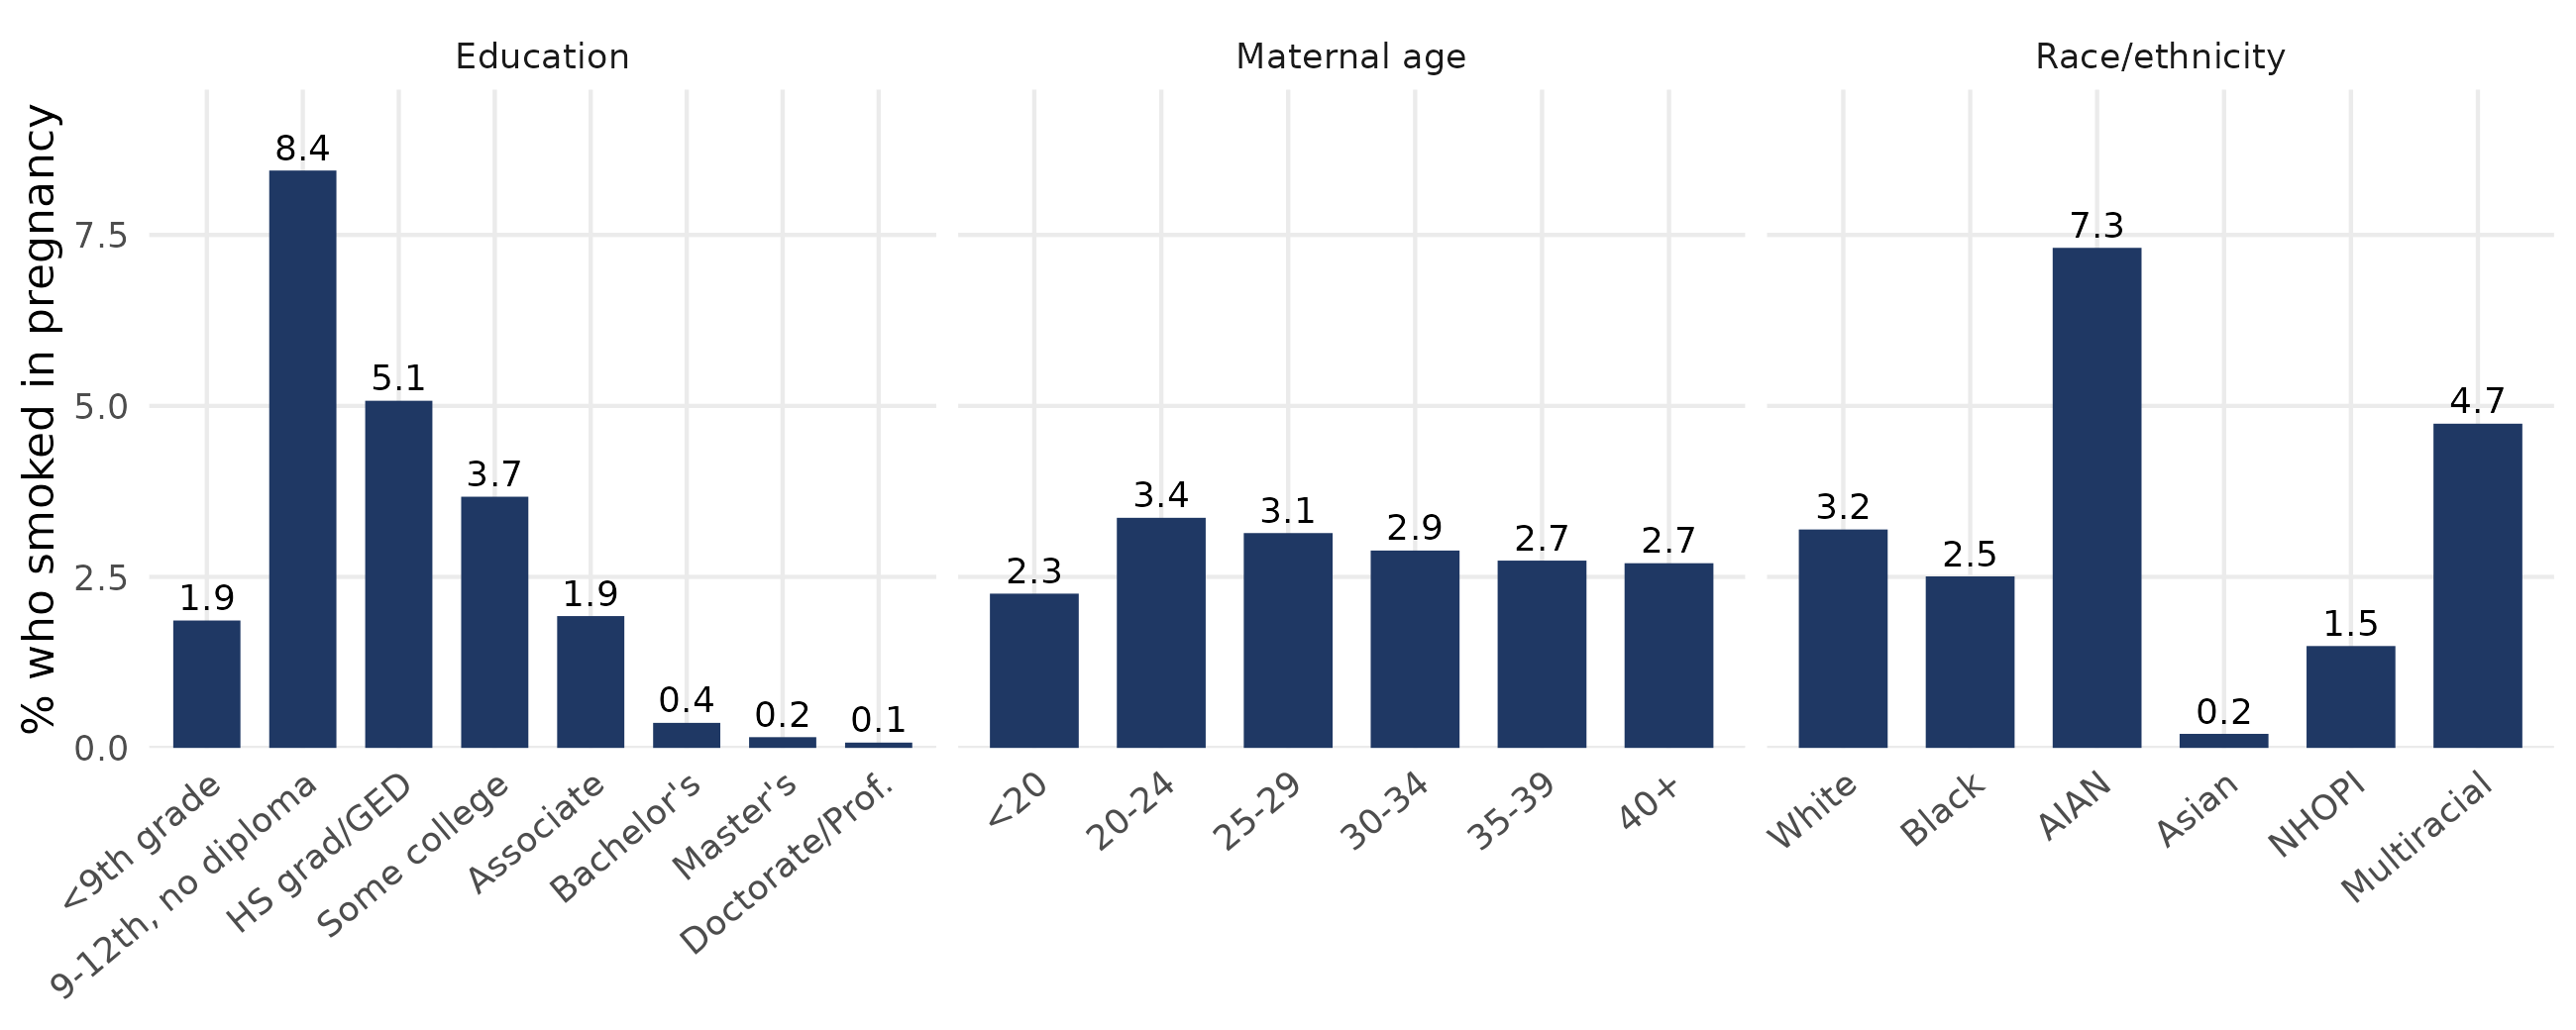
\includegraphics[width=6.4in]{figures/fig_eda_who_smokes.png}
\caption*{\textbf{Figure 1.} \emph{Percentage of mothers who smoked during pregnancy, by education, maternal age and race/ethnicity (2023 U.S. singleton births, $n = 3{,}259{,}496$).}}
\end{figure}


\begin{figure}[htbp]
\centering
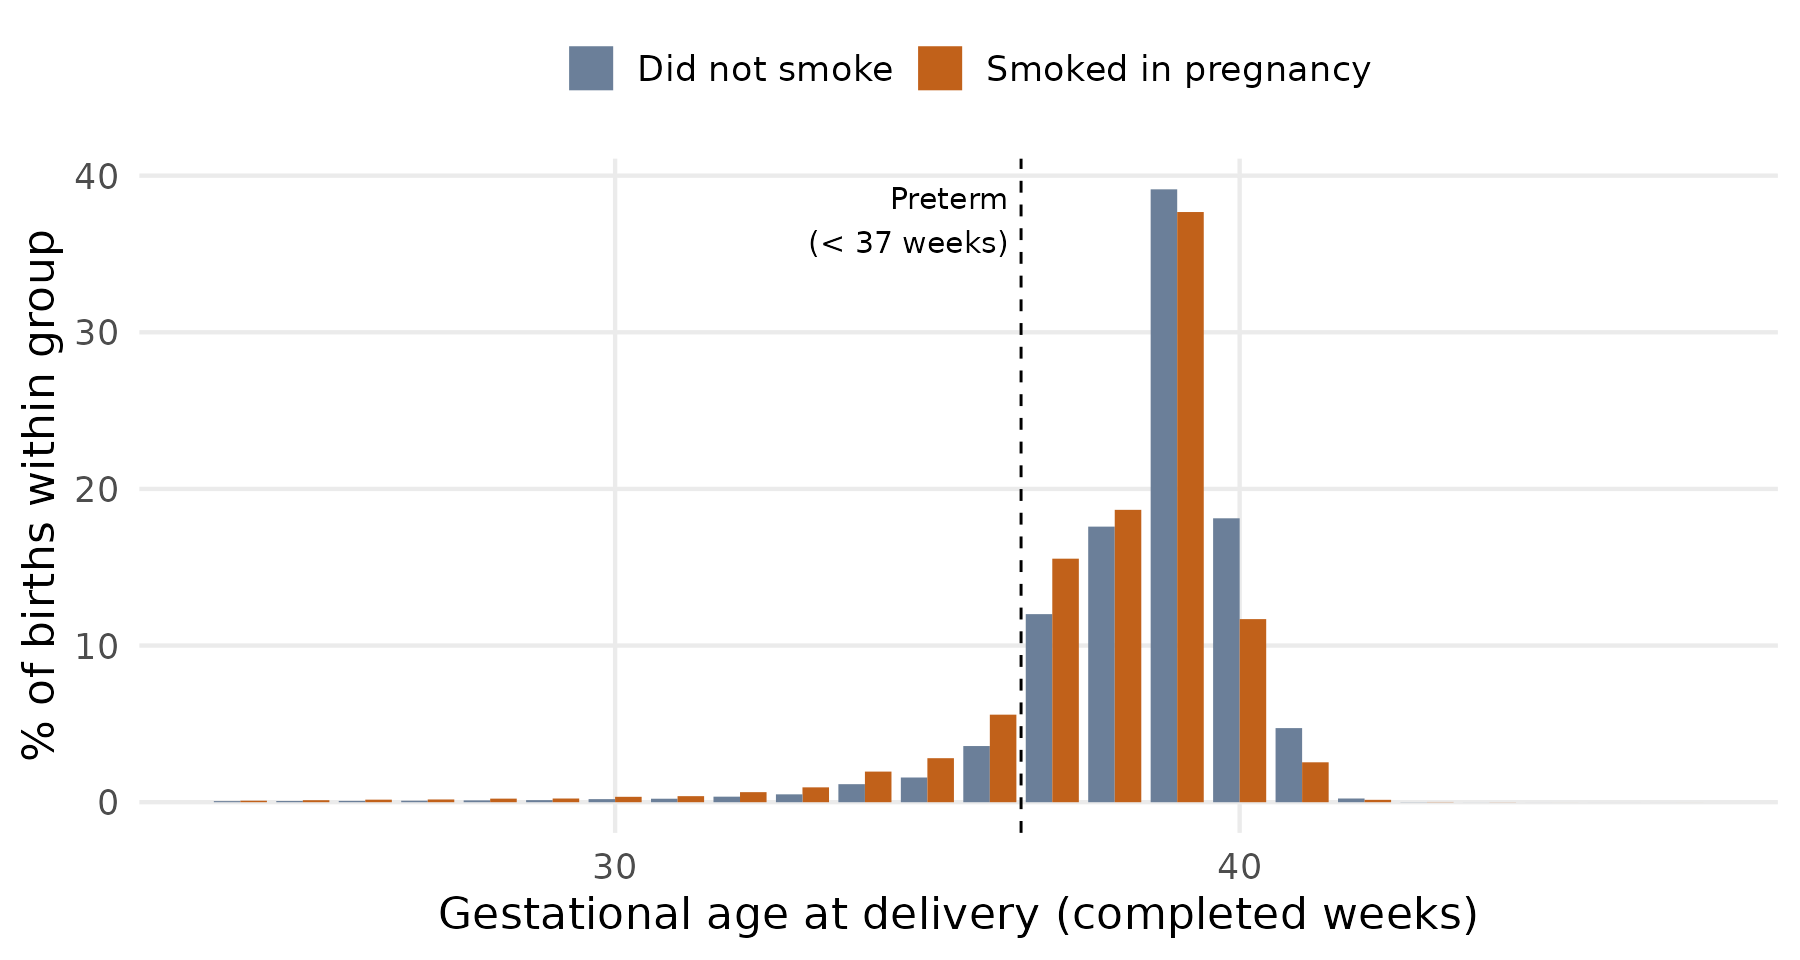
\includegraphics[width=4.9in]{figures/fig_eda_gestational_age.png}
\caption*{\textbf{Figure 2.} \emph{Distribution of gestational age at delivery by smoking status. The dashed line marks 37 weeks.}}
\end{figure}


\section*{4. Causal framework}

\subsection*{4.1 Estimand and assumptions}

Let $T$ be smoking during pregnancy, $Y$ preterm birth, and $Y(1)$ and $Y(0)$ the potential outcomes if the mother had smoked or not (Rubin, 1974). The primary estimand is the average treatment effect on the risk difference scale:
\begin{equation}
\mathrm{ATE} = \mathbb{E}[Y(1)] - \mathbb{E}[Y(0)],
\end{equation}
which is the difference in preterm risk if every mother in the cohort smoked against if none did. The ratio and odds ratio versions are also reported, together with the average effect among mothers who smoked (ATT). Identification rests on four assumptions. Conditional exchangeability, $Y(t) \perp\!\!\!\perp T \mid X$, is argued through the causal diagram below and cannot be tested. Positivity, $0 < P(T = 1 \mid X) < 1$, is assessed with the propensity score distribution (Section 6.2). Consistency means that the observed outcome equals the potential outcome under the observed exposure; here ``any smoking'' combines different doses and timing, so it holds only for that coarse exposure, and no interference between mothers is assumed. The fourth condition belongs to the estimator: AIPTW is consistent if either the propensity model or the outcome model is correctly specified (Bang \& Robins, 2005; Funk et al., 2011).

\subsection*{4.2 The causal diagram}

The diagram was built from published evidence for each arrow, following the recommendation to document every edge of an applied DAG (Tennant et al., 2021; Ferguson et al., 2020) and the standard graphical criterion for adjustment (Pearl, 1995; Greenland et al., 1999). The diagram (Figure 3) has smoking ($T$) and preterm birth ($Y$) and ten confounders, each a parent of both. That gives ten back-door paths, $T \leftarrow X \rightarrow Y$, and adjusting for all ten blocks every one of them. Table 2 gives the evidence for each arrow into T and into Y and states how strong that evidence is, because for several arrows into T it is indirect. Arrows among the confounders (dashed in Figure 3, Table 3) are assumed relationships; they do not change the minimal sufficient adjustment set, because every confounder is a direct parent of T and so each back-door path is blocked at its first node, whatever arrows connect the confounders to each other.

\begin{figure}[htbp]
\centering
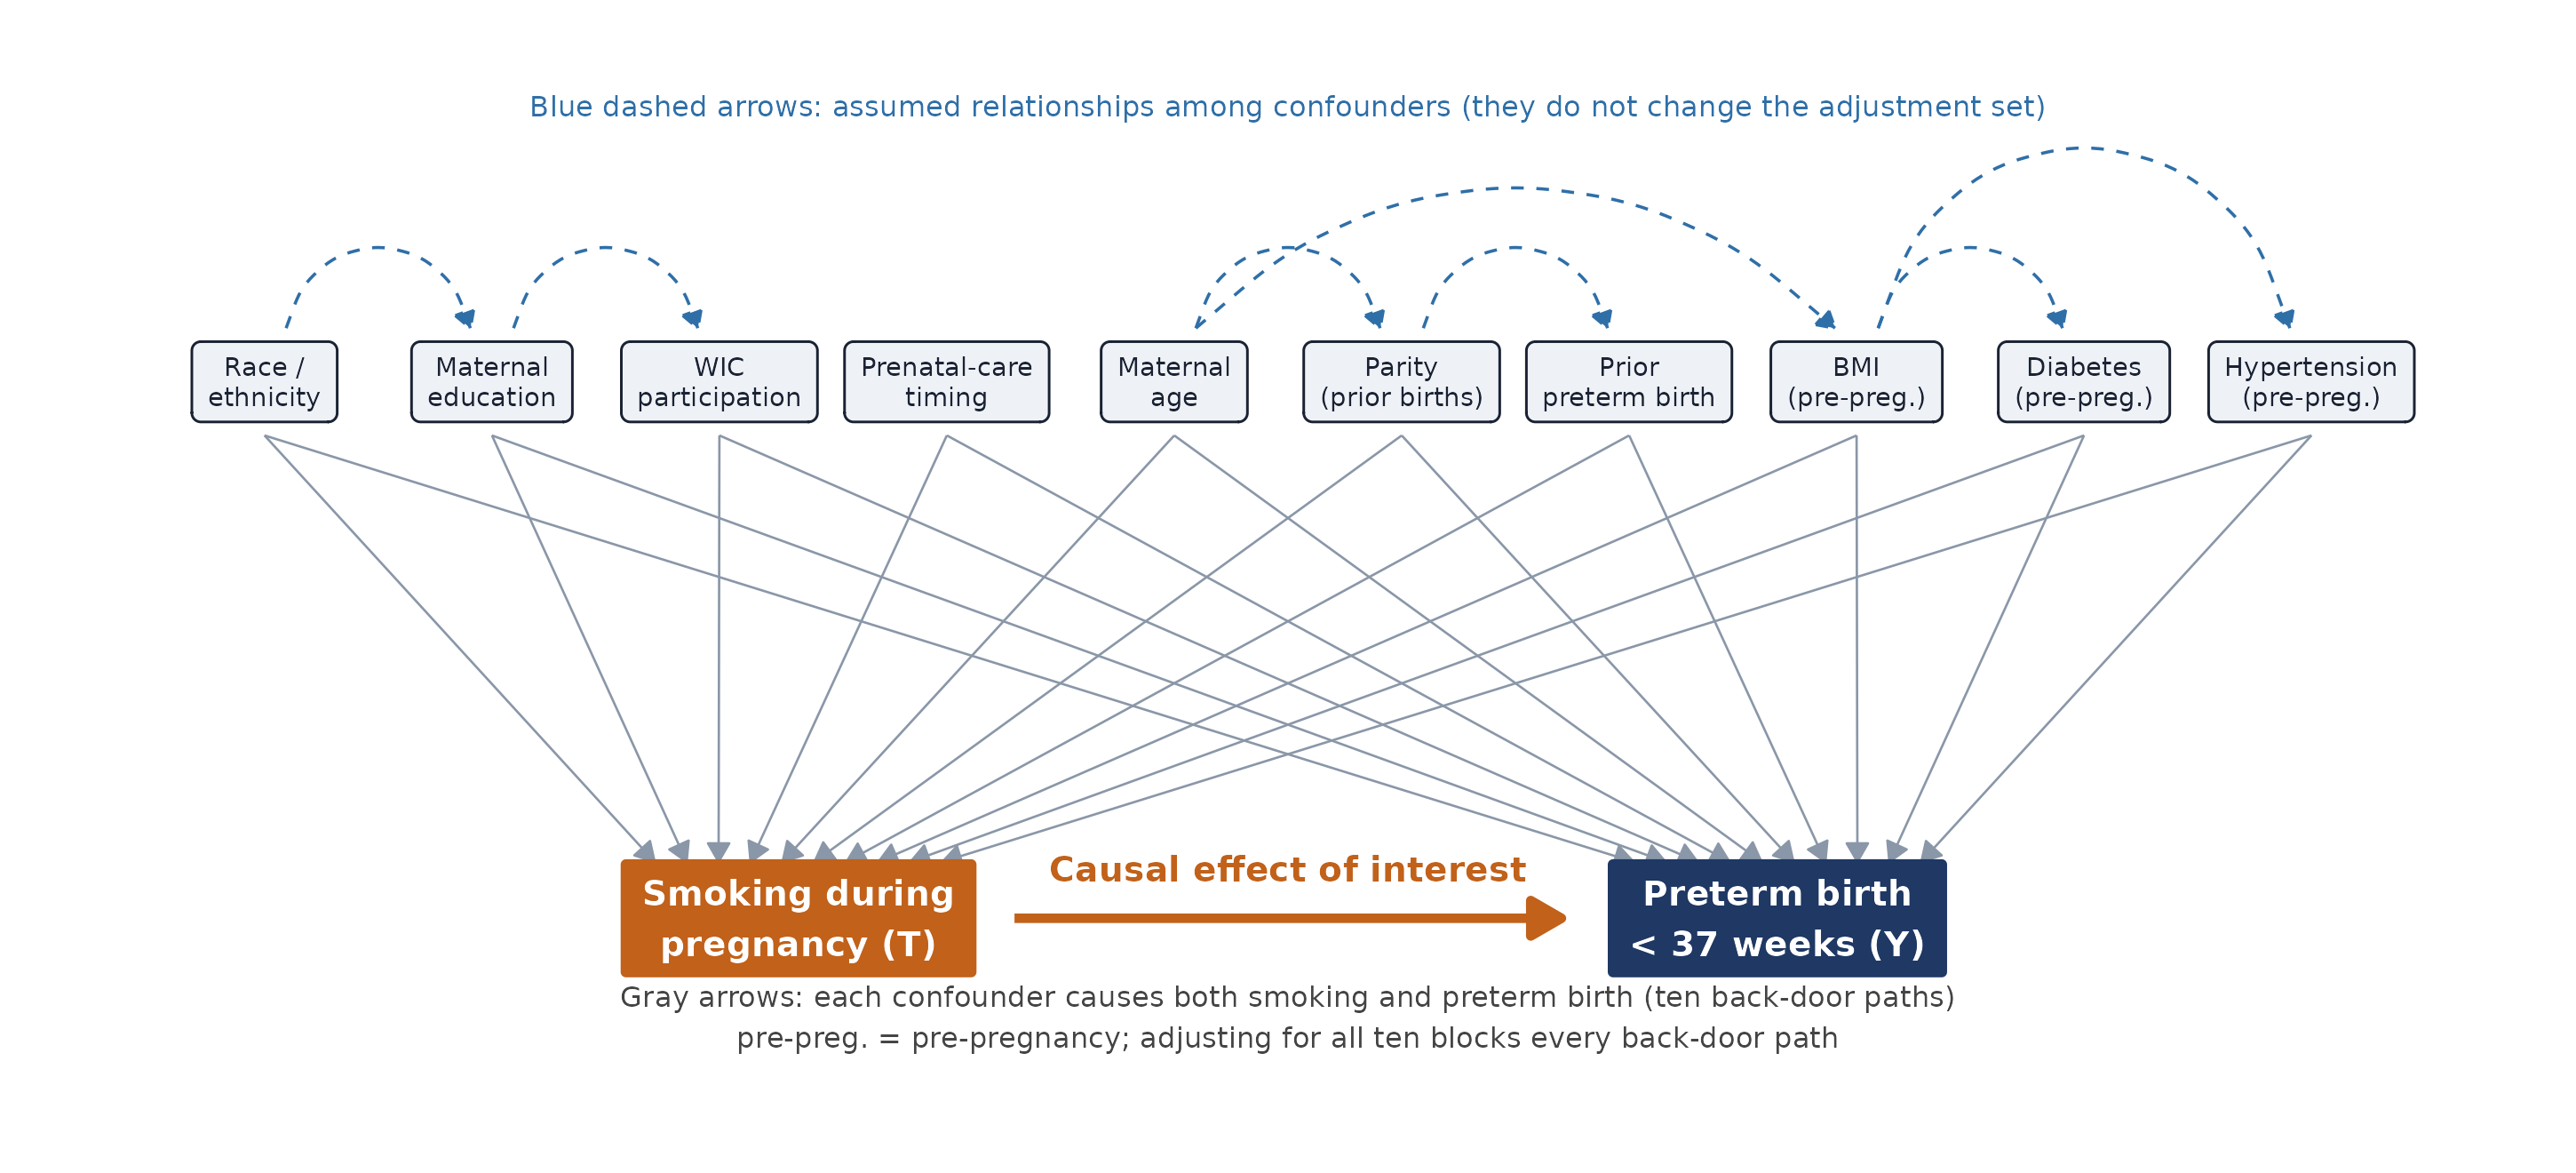
\includegraphics[width=6.5in]{figures/fig_dag.png}
\caption*{\textbf{Figure 3.} \emph{Causal diagram. Orange: exposure ($T$). Navy: outcome ($Y$). Gray arrows: each confounder affects both T and Y. Blue dashed arrows: assumed relationships among confounders. Pre-preg. = pre-pregnancy.}}
\end{figure}


Three points deserve emphasis because they are where an applied diagram is most open to challenge. First, several arrows into smoking are documented as associations or are included as proxies for shared upstream causes rather than as direct causal effects (diabetes, hypertension, previous preterm birth, parity, and in part BMI). They stay in the set because each is a documented cause or strong predictor of preterm birth (Table 2); their relation to smoking is indirect, as Table 2 states. This follows the rule of adjusting for covariates that cause the exposure, the outcome or both (VanderWeele \& Shpitser, 2011), and adjusting for strong predictors of the outcome reduces variance in propensity score analyses (Brookhart et al., 2006). Second, prenatal-care timing and WIC are recorded during pregnancy, so they can be influenced by smoking history and by the length of the pregnancy itself, which is a gestational age bias (Shin \& Song, 2019; Heaman et al., 2008; Joyce et al., 2008; Stoner et al., 2018). They are kept in the main model as markers of access and socioeconomic position, and the result without them is shown (sensitivity analysis A), because adjusting for variables downstream of the exposure can bias the estimate (Schisterman et al., 2009; Cole et al., 2010; Hernán et al., 2004). Third, health insurance type was left out of the main model. Payer on the birth certificate is recorded at delivery, and no study establishing an effect of insurance on smoking in pregnancy was identified in the literature reviewed for this paper. Insurance enters only in sensitivity analysis B. Conditions that arise during the pregnancy (gestational diabetes and hypertension) were not adjusted for because they come after smoking in time, and pre-pregnancy cigarettes per day was not adjusted for because it is closely related to the exposure itself; the latter is a design choice listed among the limitations.

{\scriptsize
\begin{longtable}{>{\raggedright\arraybackslash}p{0.151\textwidth}>{\raggedright\arraybackslash}p{0.395\textwidth}>{\raggedright\arraybackslash}p{0.395\textwidth}}
\caption*{\textbf{Table 2.} \emph{Evidence for each arrow from a confounder into smoking ($T$) and into preterm birth ($Y$). ``Documented'' means a statistic or study was found for the arrow; ``proxy'' means the variable is included as a marker of shared causes, with no direct causal study found.}}\\
\toprule
\rowcolor{headgray} \textbf{Confounder} & \textbf{Arrow into smoking ($T$)} & \textbf{Arrow into preterm birth ($Y$)} \\
\midrule
\endfirsthead
\toprule
\rowcolor{headgray} \textbf{Confounder} & \textbf{Arrow into smoking ($T$)} & \textbf{Arrow into preterm birth ($Y$)} \\
\midrule
\endhead
\bottomrule
\endfoot
Maternal age & Documented. Non-monotone: 10.7\% at ages 20-24, 2.0\% at 45 and over (2016 birth certificates) (Drake et al., 2018; Kondracki, 2019; Tong et al., 2013). & Documented. Lowest preterm rate at 25-29 (9.28\%), highest at 40 and over (14.59\%) in 2017 (Martin et al., 2018); higher risk in adolescent mothers in a WHO multicountry study (Ganchimeg et al., 2014). \\
Race and ethnicity & Documented. Prevalence differs several-fold (2016: American Indian and Alaska Native 16.7\%, Asian 0.6\%) (Drake et al., 2018); 2023: White 4.4\%, Black 2.7\%, Hispanic 0.8\% (Osterman et al., 2025). Race stands for social and structural processes, not biology (Phelan \& Link, 2015; VanderWeele \& Robinson, 2014). & Documented. 2023 preterm rates: Black 14.65\%, Hispanic 10.14\%, White 9.44\%, Asian 9.08\% (Osterman et al., 2025); structural factors explain about half of the Black-White gap in one U.S. analysis (Gangopadhyaya et al., 2024). \\
Education & Documented. 12.2\% (high school) and 11.7\% (less than high school) against at most 1.0\% (bachelor's or higher) among women 25 and over (Drake et al., 2018); Mendelian randomization supports a causal effect of education on smoking (Gage et al., 2018); reviewed in (Hiscock et al., 2012). & Documented in European data. Low maternal education: relative excess risk 1.48 (95\% CI 1.29 to 1.69) in 12 cohorts (Ruiz et al., 2015). The U.S. gradient is shown from these data in Table A1. \\
Prenatal-care timing & Documented, but care leads to smoking: early care raised the relative risk of early cessation by 52\% in over one million Ohio births (Moore et al., 2016). Post-baseline; see text. & Documented, with gestational age bias: later or inadequate care is associated with preterm birth, but shorter pregnancies have less time to accumulate care (Shin \& Song, 2019; Heaman et al., 2008). \\
WIC participation & Plausible, weakest evidence. WIC enrollees smoked more at intake, while earlier enrollment was associated with quitting (Yunzal-Butler et al., 2009). WIC eligibility is income-based (USDA, n.d.). & Documented association with better outcomes after adjustment (Bitler \& Currie, 2005), with a gestational age bias caution (Joyce et al., 2008). \\
Parity & Proxy. No U.S. causal study of parity and smoking in pregnancy was found. & Documented, U-shaped. Nulliparity: odds ratio 1.95 for spontaneous preterm birth in 802,119 Dutch pregnancies (Koullali et al., 2020); parity of three or more raised the odds in low- and middle-income cohorts (Kozuki et al., 2013). Modelled as categories. \\
Previous preterm birth & Proxy. No study of previous preterm birth as a cause of smoking in pregnancy was found. & Documented, the strongest arrow. Recurrence of about 20\% after a previous preterm singleton (Kazemier et al., 2014). \\
Pre-pregnancy diabetes & Proxy. No study of diabetes as a cause of smoking in pregnancy was found. & Documented. 42.5\% of type 1 and 23.4\% of type 2 pregnancies delivered before 37 weeks in a UK national cohort (Murphy et al., 2021). Excess-risk interaction with smoking reported (Borsari et al., 2018); see subgroups. \\
Pre-pregnancy hypertension & Proxy. No study of hypertension as a cause of smoking in pregnancy was found. & Documented. Pooled preterm delivery 28.1\% (95\% CI 22.6 to 34.4), 2.7-fold higher than the general population (Bramham et al., 2014). \\
Pre-pregnancy BMI & Plausible, contestable. Mendelian randomization in general adult populations: higher BMI raised the odds of smoking (odds ratio 1.18 per standard deviation) (Carreras-Torres et al., 2018). The reverse arrow, smoking to weight, is also documented (Aubin et al., 2012). & Documented, heterogeneous. Null overall (RR 1.06, 95\% CI 0.87 to 1.30), with increased induced preterm birth in obesity (McDonald et al., 2010); lower spontaneous preterm risk in overweight and class I obesity, highest very-preterm risk in class III obesity (Torloni et al., 2009). Modelled as categories. \\
\end{longtable}
}


{\scriptsize
\begin{longtable}{>{\raggedright\arraybackslash}p{0.231\textwidth}>{\raggedright\arraybackslash}p{0.709\textwidth}}
\caption*{\textbf{Table 3.} \emph{Assumed arrows among confounders (dashed in Figure 3). None changes the adjustment set.}}\\
\toprule
\rowcolor{headgray} \textbf{Arrow} & \textbf{Reason and evidence} \\
\midrule
\endfirsthead
\toprule
\rowcolor{headgray} \textbf{Arrow} & \textbf{Reason and evidence} \\
\midrule
\endhead
\bottomrule
\endfoot
Race to education & Attainment gaps by race are large (bachelor's attainment at ages 25 to 29 in 2022: Asian 72\%, White 45\%, Black 28\%, Hispanic 25\%) (NCES, 2023); racism as a fundamental cause of differences in socioeconomic position (Phelan \& Link, 2015). \\
Education to WIC & WIC eligibility is income-based (USDA, n.d.). Education is assumed here to act through income; no pregnancy-specific source was reviewed for this arrow. \\
Age to parity & Older mothers have had more time to accumulate births (Mathews \& Hamilton, 2016); nearly definitional. \\
Age to BMI & Weaker and non-monotone: among pregnant women in 2019, obesity was 20.5\% under age 20 and about 30\% at ages 20 to 29 and 40 and over (Driscoll \& Gregory, 2020). \\
Parity to previous preterm birth & Structural: a mother cannot have a previous preterm birth without a previous birth. \\
BMI to diabetes and to hypertension & Relative risk of incident type 2 diabetes 12.41 and of hypertension 2.42 in obese against normal-weight women in adult cohorts (Guh et al., 2009); not pregnancy-specific. \\
\end{longtable}
}


An arrow from WIC to prenatal-care timing was considered and not drawn: for most women prenatal care registration comes before WIC enrollment, so the evidence points the other way, and the direction does not change which variables must be adjusted for (Yunzal-Butler et al., 2009). Race is treated as a node that carries social processes, as recommended for causal interpretation of race in regression (VanderWeele \& Robinson, 2014). The diagram is a statement of assumptions, not a finding of the data.

\section*{5. Methods}

\subsection*{5.1 Estimators}

Let $e(X) = P(T = 1 \mid X)$ be the propensity score (Rosenbaum \& Rubin, 1983) and $\mu_t(X) = P(Y = 1 \mid T = t, X)$ the outcome regressions, $t \in \{0, 1\}$. All three nuisance models are logistic regressions on the ten confounders (age, BMI, and the other variables as categories, so that the models do not assume a straight line in age or BMI). Five estimators of the risk difference, risk ratio and odds ratio are reported.
\begin{enumerate}[leftmargin=2.2em,itemsep=2pt,topsep=3pt]
\item \emph{Crude:} the unadjusted contrast.
\item \emph{Outcome regression (g-computation):} the average of $\hat\mu_1(X)$ and $\hat\mu_0(X)$ over all births (Naimi et al., 2017),
\begin{equation}\hat\psi_t^{\mathrm{OR}} = \frac{1}{n}\sum_{i=1}^{n}\hat\mu_t(X_i).\end{equation}
\item \emph{Stabilized inverse probability of treatment weighting (IPTW)} with normalized (H\'ajek) weights $w_i = P(T = t)\,/\,P(T = t \mid X_i)$ (Austin \& Stuart, 2015),
\begin{equation}\hat\psi_t^{\mathrm{IPTW}} = \frac{\sum_{i:\,T_i = t} w_i\,Y_i}{\sum_{i:\,T_i = t} w_i}.\end{equation}
\item \emph{Propensity score stratification} into quintiles with a Mantel-Haenszel odds ratio (Rosenbaum \& Rubin, 1984).
\item \emph{AIPTW, the primary estimator} (Robins et al., 1994; Bang \& Robins, 2005; Funk et al., 2011):
\begin{align}
\hat\psi_1^{\mathrm{AIPTW}} &= \frac{1}{n}\sum_{i=1}^{n}\left[\hat\mu_1(X_i) + \frac{T_i\,\big(Y_i - \hat\mu_1(X_i)\big)}{\hat e(X_i)}\right],\\
\hat\psi_0^{\mathrm{AIPTW}} &= \frac{1}{n}\sum_{i=1}^{n}\left[\hat\mu_0(X_i) + \frac{(1 - T_i)\,\big(Y_i - \hat\mu_0(X_i)\big)}{1 - \hat e(X_i)}\right],
\end{align}
with $\widehat{\mathrm{ATE}} = \hat\psi_1^{\mathrm{AIPTW}} - \hat\psi_0^{\mathrm{AIPTW}}$.
\end{enumerate}
AIPTW starts from the outcome-model prediction for every mother and corrects it with the inverse-probability-weighted residual of the mothers who actually had that exposure. If the outcome model is right, the correction averages to zero; if only the propensity model is right, the correction removes the bias of the outcome model (Bang \& Robins, 2005).

\subsection*{5.2 Why weighting and not matching}

The propensity score is used to weight, for four reasons. Weighting keeps all 3,259,496 births, whereas matching discards unmatched births and changes the population to which the estimate applies (Stuart, 2010). Weighting targets the population average effect directly, which is the estimand stated above. Matching on the propensity score can increase imbalance, inefficiency, model dependence and bias (King \& Nielsen, 2019), and finite-sample comparisons of reweighting and matching estimators are an active literature (Busso et al., 2014; Stuart, 2010). And with 3.26 million births and a 3 percent exposure, weighting is computationally direct, with variances available from the influence function rather than from a resampling scheme alone. The cost is that weighting is sensitive to very small propensity scores, which is addressed with clamping, diagnostics and sensitivity analyses.

\subsection*{5.3 Inference, extreme weights and overlap weights}

Each estimator is an average of per-birth values, $\hat\psi = n^{-1}\sum_{i=1}^{n}\hat\psi_i$, and its standard error comes from the estimated influence function,
\begin{equation}
\widehat{\mathrm{SE}}(\hat\psi) = \sqrt{\widehat{\mathrm{Var}}(\hat\psi_i)\,/\,n},
\end{equation}
with the delta method for the risk ratio and odds ratio. The 95 percent confidence intervals are Wald intervals. These ignore uncertainty in the propensity and outcome models, as is conventional for AIPTW with parametric nuisance models (Funk et al., 2011); a bootstrap on a subsample, described in Section 6.6, checks them. Because a large share of non-smokers have a very low estimated probability of smoking, a few smokers receive large weights. In the main analysis the propensity score is clamped (rather than deleted) at its 1st and 99th percentiles, which bounds the largest weight; weight trimming can improve precision with a logistic propensity model but is no substitute for a well specified one (Lee et al., 2011), and doubly robust estimators remain sensitive to small estimated propensities (Kang \& Schafer, 2007), so results with no truncation, with truncation at the 0.1/99.9 and 5/95 percentiles, and with deletion of births outside a propensity range of 0.01 to 0.99 are also reported (Section 6.4). As an additional check, overlap-weighted effects are estimated; they target the population with the most overlap and give bounded weights (Li et al., 2018). The ATT by AIPTW is also reported; it requires weights only for non-smokers:
\begin{equation}
\widehat{\mathrm{ATT}} = \frac{\sum_{i=1}^{n}\Big[T_i\big(Y_i-\hat\mu_0(X_i)\big) - (1-T_i)\,\dfrac{\hat e(X_i)}{1-\hat e(X_i)}\big(Y_i-\hat\mu_0(X_i)\big)\Big]}{\sum_{i=1}^{n}T_i}.
\end{equation}

\subsection*{5.4 Sensitivity analyses, subgroups and unmeasured confounding}

The AIPTW risk difference was re-estimated under four alternative covariate specifications: (A) only pre-pregnancy confounders, dropping prenatal-care timing and WIC; (B) the main set plus insurance type; (C) age and BMI as continuous variables with quadratic terms; and (D) the main set plus two-way interactions (race by education, age by education, age by parity, education by WIC, education by prenatal care). To examine whether the effect differs between groups, AIPTW was estimated within subgroups of age, race and ethnicity, education, BMI, parity and previous preterm birth, and these estimates are treated as exploratory. For unmeasured confounding, the E-value is reported: the minimum risk ratio association that an unmeasured confounder would need with both smoking and preterm birth, beyond the measured confounders, to explain the observed risk ratio away (VanderWeele \& Ding, 2017); for a risk ratio $\mathrm{RR} > 1$ it is
\begin{equation}
E\text{-value} = \mathrm{RR} + \sqrt{\mathrm{RR}\,(\mathrm{RR} - 1)}.
\end{equation}

\subsection*{5.5 Software and reproducibility}

All analyses were run in R 4.3.3 with base R and the data.table package; figures use ggplot2. To keep the code runnable on a standard laptop and independent of package versions, the logistic regressions are fitted by iteratively reweighted least squares in base R, processed in chunks; a self-test in the code confirms they match glm() to within 5e-6. Every random operation uses set.seed(1234). The scripts are numbered in run order (00 optional data extraction, 01 data preparation, 02 exploratory analysis, 03 main analysis, 04 sensitivity analyses, 05 variance check, 06 causal diagram, 07 numbers quoted in the text), and each states its inputs, outputs and run time at the top. The data link and download instructions are at the top of scripts 00 and 01.

\section*{6. Results}

\subsection*{6.1 Unadjusted comparison}

In the analytic cohort the crude preterm risk was 13.90 percent among mothers who smoked and 8.30 percent among those who did not, a crude risk difference of 5.60 (5.38, 5.82) percentage points, a risk ratio of 1.68 (1.65, 1.70) and an odds ratio of 1.78 (1.75, 1.82) (Table 4).

\subsection*{6.2 Overlap and covariate balance}

The propensity score separates the two groups only partly (Figure 4). The median estimated probability of smoking was 0.058 among smokers and 0.018 among non-smokers, and 40.8 percent of non-smokers had a score below 0.01, indicating that a large share of non-smokers have a very low estimated probability of smoking. Only 4.1 percent of smokers had a score below 0.01. The 1st and 99th percentiles used for clamping were 0.0002 and 0.163. Because the target is the whole cohort, smokers with low scores carry large weights: after clamping, the largest stabilized weight among smokers was 187, the top 1 percent of smokers carried 23.2 percent of the total smoker weight, and the effective sample size of the weighted smokers was 6,807 of 97,187. The weights among non-smokers were close to one (range 0.97 to 1.16). This limits the precision of the ATE estimate; the ATT and overlap-weighted results are shown alongside it.

Weighting reduced imbalance (Figure 5). The largest absolute standardized mean difference fell from 0.64 before weighting (bachelor's degree) to 0.13 after, and 3 of 38 covariate levels remained above the conventional 0.10 threshold: age 40+ (0.10), Asian (0.11), BMI 18.5-24.9 (0.13). These levels are reported as residual imbalance after weighting (Austin \& Stuart, 2015).

\begin{figure}[htbp]
\centering
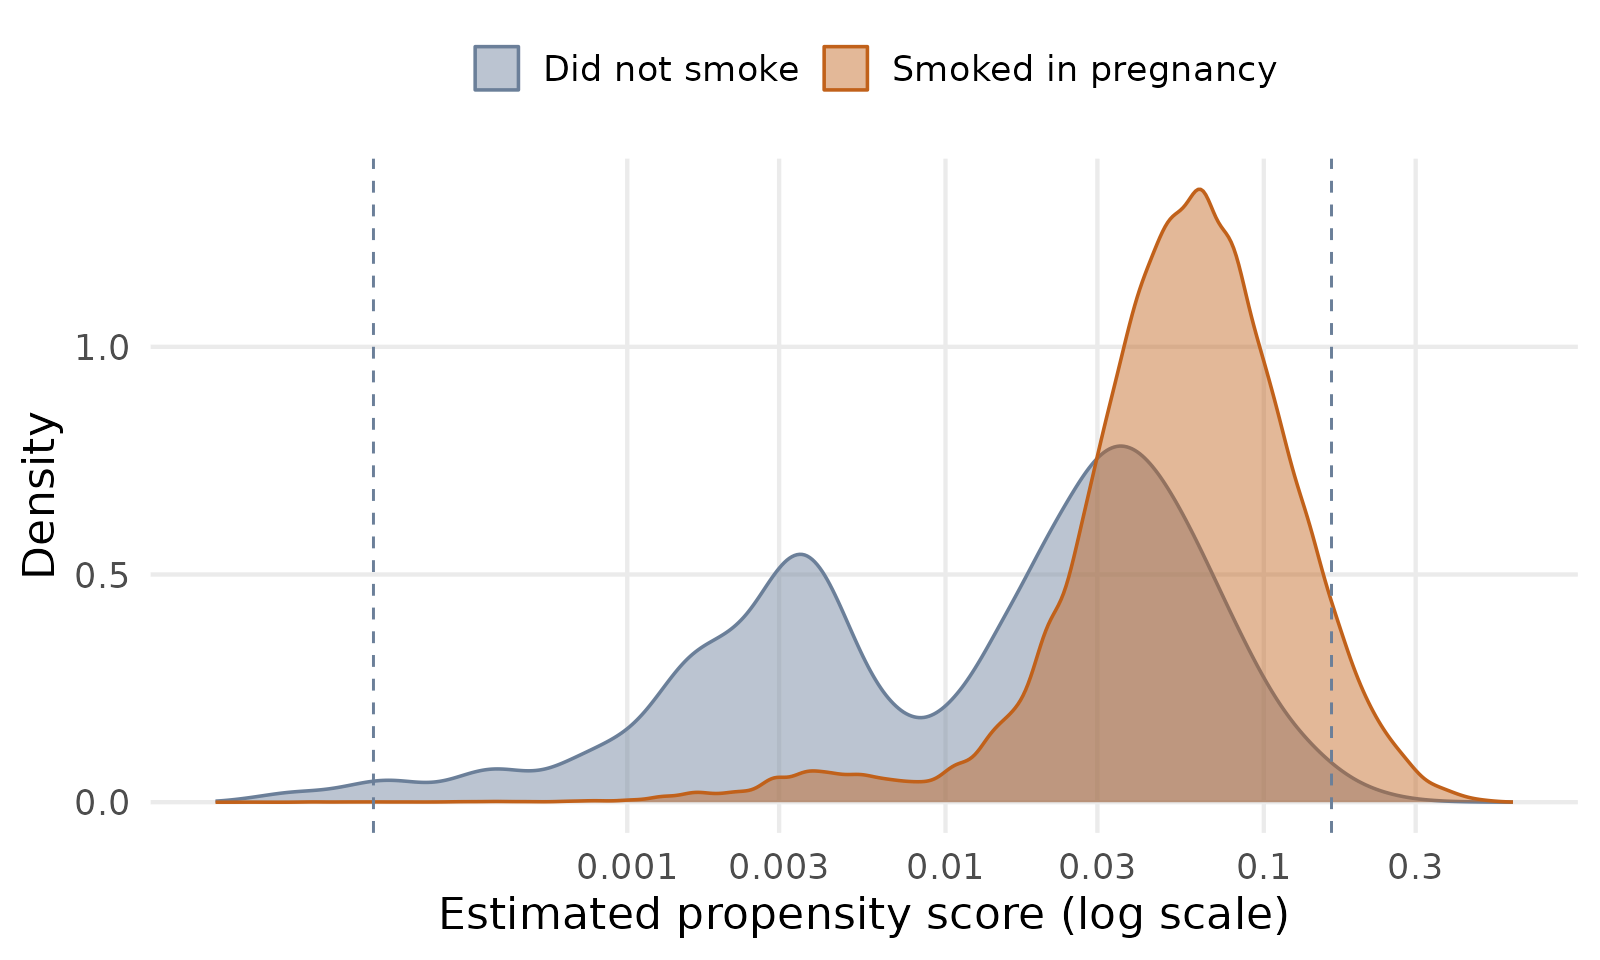
\includegraphics[width=5.4in]{figures/fig_ps_overlap.png}
\caption*{\textbf{Figure 4.} \emph{Estimated propensity score (probability of smoking given the ten confounders) by smoking status, log scale. Dashed lines mark the 1st and 99th percentiles at which the score is clamped.}}
\end{figure}


\begin{figure}[htbp]
\centering
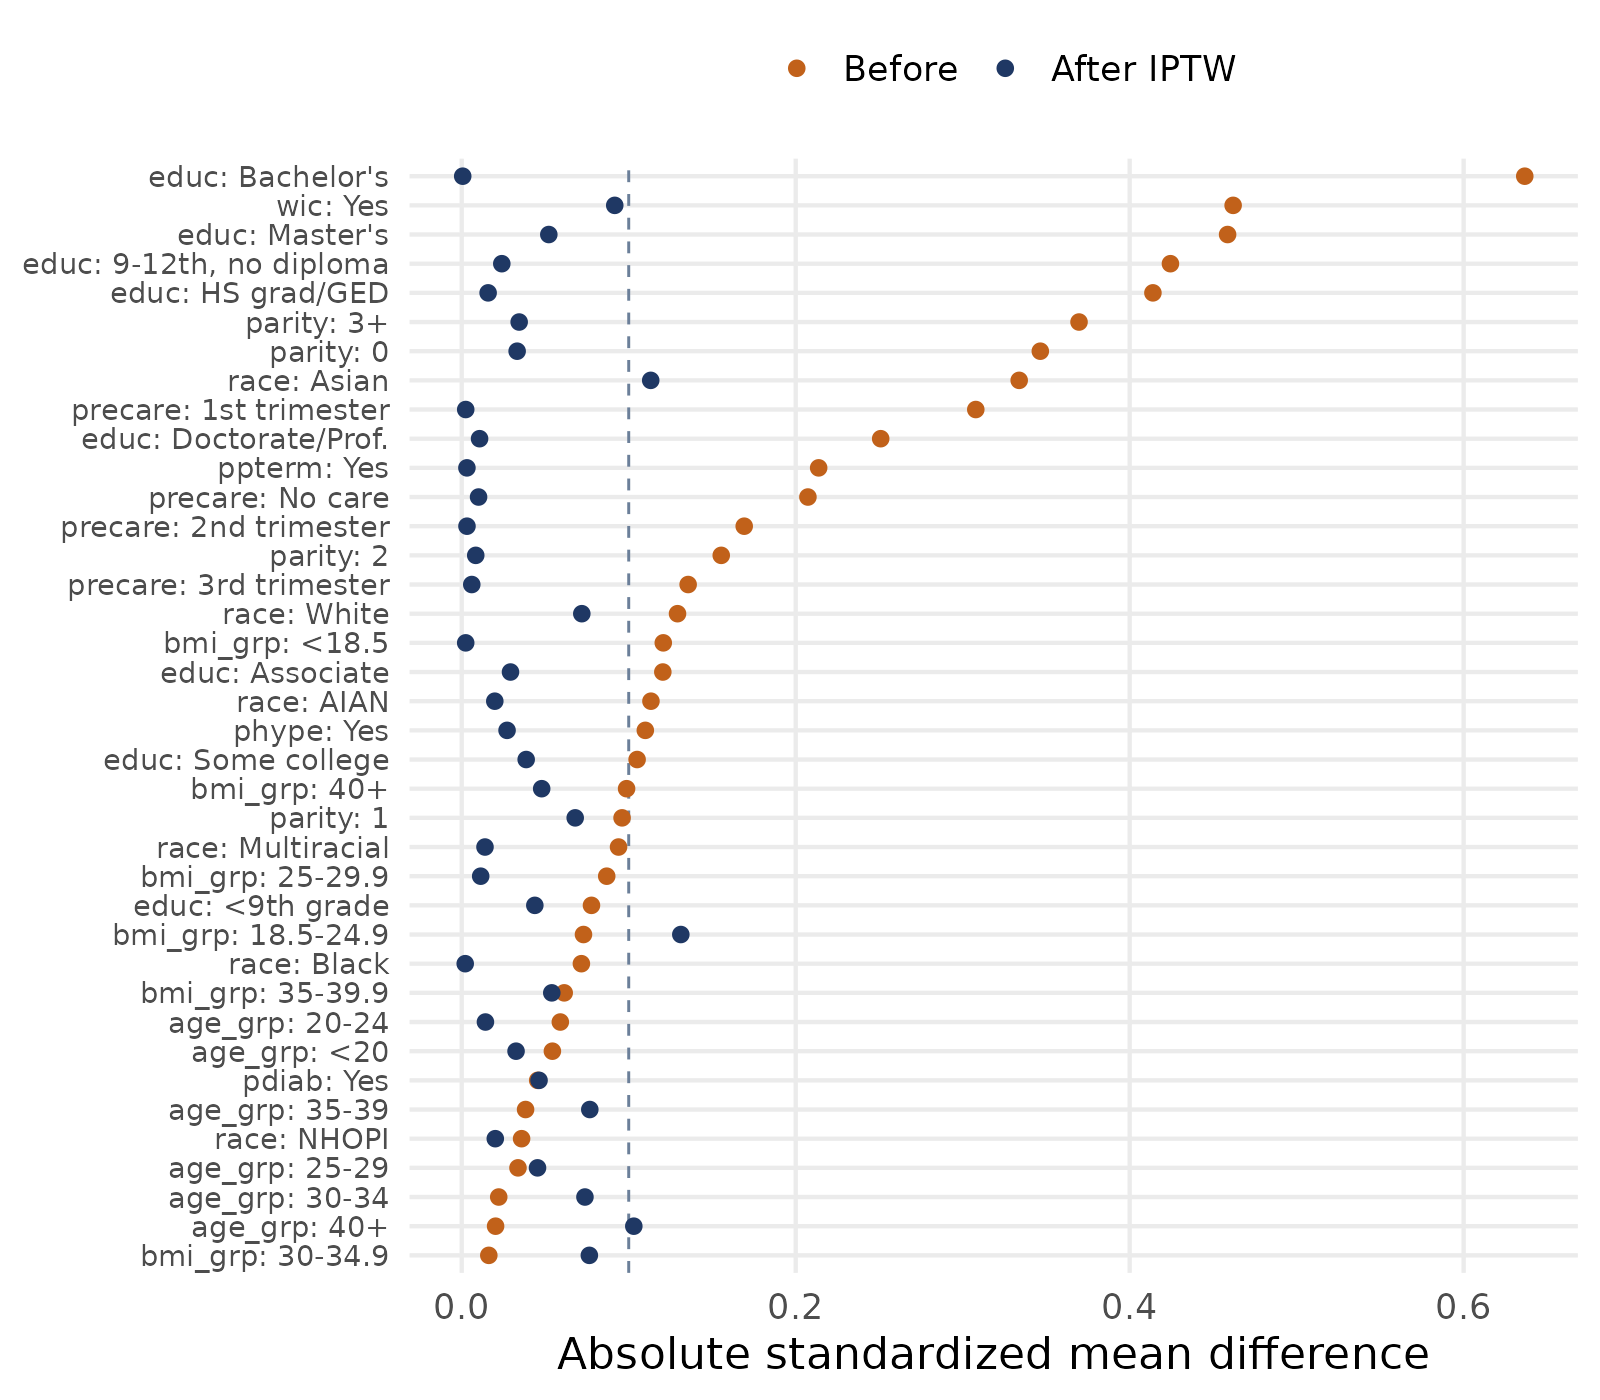
\includegraphics[width=4.9in]{figures/fig_love_plot.png}
\caption*{\textbf{Figure 5.} \emph{Absolute standardized mean differences for all covariate levels before and after stabilized inverse probability weighting. Dashed line: 0.10.}}
\end{figure}


\subsection*{6.3 Effect estimates}

The four adjusted estimators gave risk differences between 3.26 and 3.74 percentage points (Table 4, Figure 6). The AIPTW risk difference was 3.26 (2.47, 4.04) percentage points, with standardized preterm risks of 11.62 percent if every mother smoked and 8.37 percent if none did, a risk ratio of 1.39 (1.30, 1.49) and an odds ratio of 1.44 (1.33, 1.55). Outcome regression gave 3.48, stabilized IPTW 3.53 and propensity score stratification 3.74 percentage points. Adjustment therefore reduced the crude risk difference of 5.60 by 33 to 42 percent. The IPTW interval (2.77 to 4.30) is wider than the outcome regression interval (3.00 to 3.96). Conditional odds ratios from the usual adjusted logistic regression and from the Mantel-Haenszel combination over propensity score quintiles were 1.42 (1.39, 1.44) and 1.48 (1.45, 1.50). Among mothers who smoked, the AIPTW average effect (ATT) was 3.39 (3.17, 3.61) percentage points. Under the assumptions of Section 4, this corresponds to about 34 additional preterm births per 1,000 smoking pregnancies.

{\footnotesize
\begin{longtable}{>{\raggedright\arraybackslash}p{0.210\textwidth}>{\raggedright\arraybackslash}p{0.101\textwidth}>{\raggedright\arraybackslash}p{0.101\textwidth}>{\raggedright\arraybackslash}p{0.168\textwidth}>{\raggedright\arraybackslash}p{0.159\textwidth}>{\raggedright\arraybackslash}p{0.162\textwidth}}
\caption*{\textbf{Table 4.} \emph{Effect of smoking during pregnancy on preterm birth, 2023 U.S. singleton births ($n = 3{,}259{,}496$). Risk difference (RD) in percentage points. 95\% confidence intervals in parentheses. AIPTW is the primary estimator.}}\\
\toprule
\rowcolor{headgray} \textbf{Estimator} & \textbf{Risk if smoked (\%)} & \textbf{Risk if not (\%)} & \textbf{Risk difference} & \textbf{Risk ratio} & \textbf{Odds ratio} \\
\midrule
\endfirsthead
\toprule
\rowcolor{headgray} \textbf{Estimator} & \textbf{Risk if smoked (\%)} & \textbf{Risk if not (\%)} & \textbf{Risk difference} & \textbf{Risk ratio} & \textbf{Odds ratio} \\
\midrule
\endhead
\bottomrule
\endfoot
Crude (unadjusted) & 13.90 & 8.30 & 5.60 (5.38, 5.82) & 1.68 (1.65, 1.70) & 1.78 (1.75, 1.82) \\
Outcome regression (g-computation) & 11.84 & 8.36 & 3.48 (3.00, 3.96) & 1.42 (1.36, 1.47) & 1.47 (1.41, 1.54) \\
IPTW (stabilized) & 11.89 & 8.36 & 3.53 (2.77, 4.30) & 1.42 (1.33, 1.52) & 1.48 (1.38, 1.59) \\
PS-quintile stratification & 12.08 & 8.35 & 3.74 (3.25, 4.22) & 1.45 (1.39, 1.51) & 1.51 (1.44, 1.58) \\
AIPTW (doubly robust) & 11.62 & 8.37 & 3.26 (2.47, 4.04) & 1.39 (1.30, 1.49) & 1.44 (1.33, 1.55) \\
\end{longtable}
}


\begin{figure}[htbp]
\centering
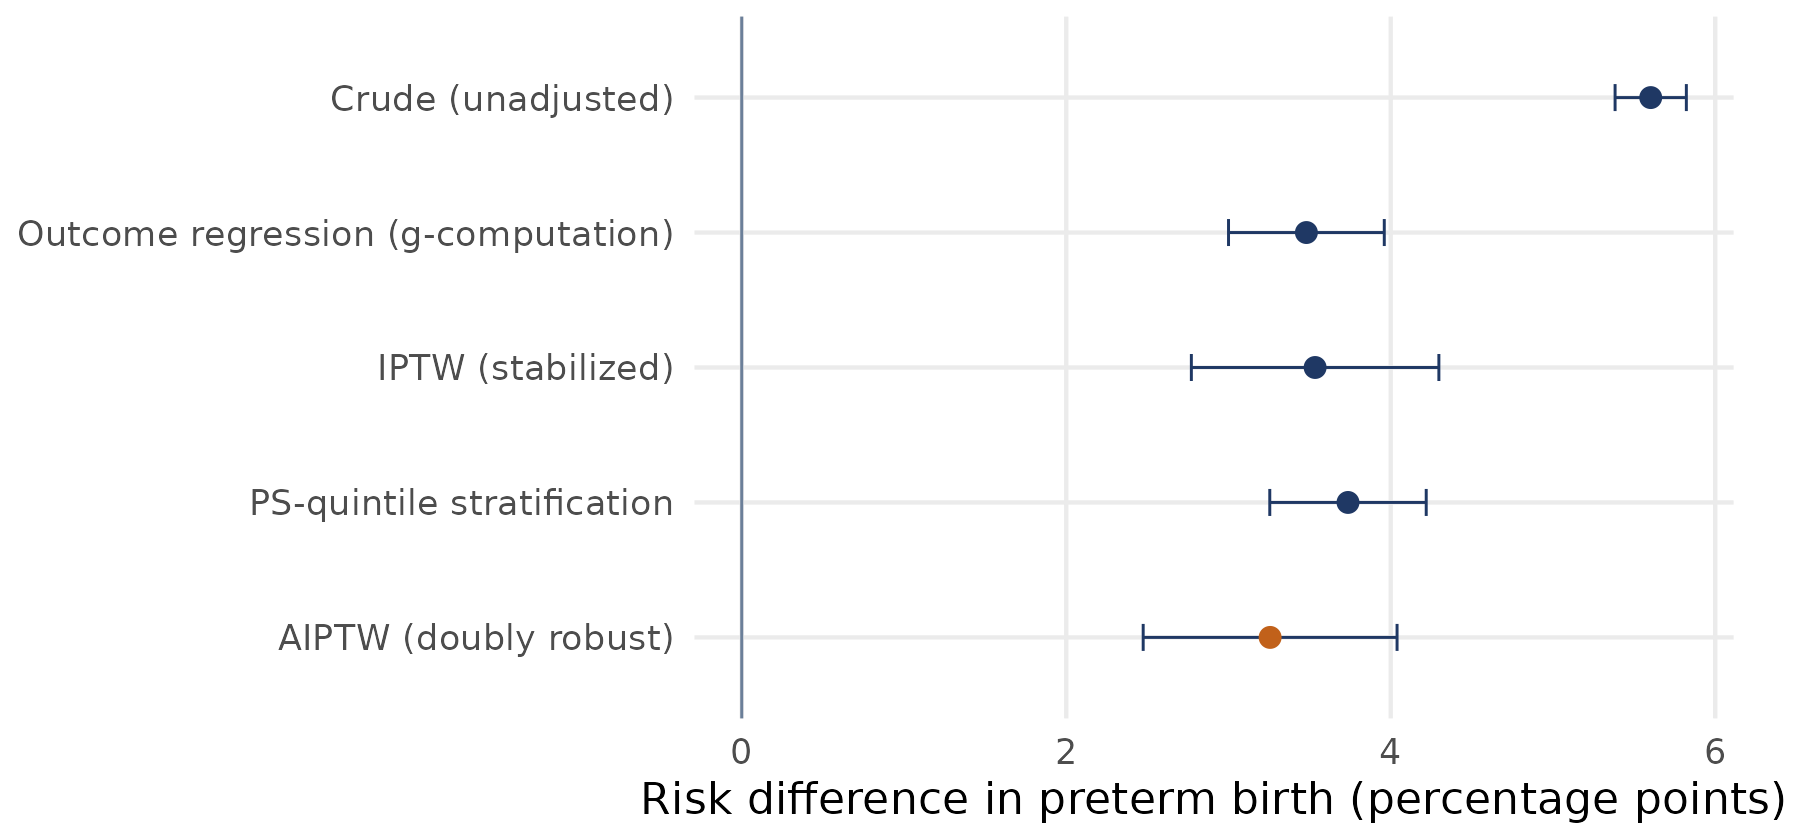
\includegraphics[width=5.4in]{figures/fig_forest_rd.png}
\caption*{\textbf{Figure 6.} \emph{Risk difference in preterm birth (percentage points) by estimator, with 95\% confidence intervals. The primary estimator (AIPTW) is in orange.}}
\end{figure}


The E-value for the AIPTW risk ratio is 2.12, and 1.92 for the lower confidence limit. An unmeasured confounder would have to be associated with both smoking and preterm birth by a risk ratio of at least about 2.1 each, beyond the ten confounders already in the model, to explain the point estimate away entirely, and by about 1.9 each to move the confidence interval to include no effect (VanderWeele \& Ding, 2017). The E-value says how strong such a confounder would need to be, not whether one exists. Alcohol, cannabis, e-cigarette use, stress and interpregnancy interval are unmeasured here and each is related to preterm birth (Patra et al., 2011; Regan et al., 2021; Dole et al., 2003; Ahrens et al., 2019).

\subsection*{6.4 Sensitivity to propensity score handling and to the covariate specification}

Table 5 shows the effect estimate under different handling of the extreme propensity scores. The AIPTW risk difference ranged from 3.03 to 3.39 percentage points across no truncation, clamping at the 0.1/99.9, 1/99 and 5/95 percentiles, deleting births with a score outside 0.01 to 0.99, and overlap weighting. Without any truncation the largest weight was 453 and the effective smoker sample 5,134. Deleting births outside the 0.01 to 0.99 range keeps only about 60 percent of the cohort, changes the population to which the estimate applies, and gives a narrower interval; it is shown for completeness and is not used as the main result. The overlap-weighted risk difference was 3.30 percentage points, within the range of the AIPTW estimates in this table.

{\scriptsize
\begin{longtable}{>{\raggedright\arraybackslash}p{0.308\textwidth}>{\raggedright\arraybackslash}p{0.111\textwidth}>{\raggedright\arraybackslash}p{0.163\textwidth}>{\raggedright\arraybackslash}p{0.144\textwidth}>{\raggedright\arraybackslash}p{0.077\textwidth}>{\raggedright\arraybackslash}p{0.097\textwidth}}
\caption*{\textbf{Table 5.} \emph{Sensitivity of the effect estimate to propensity score handling (AIPTW and overlap weighting). RD in percentage points. Max. weight and effective n (ESS) are for smokers.}}\\
\toprule
\rowcolor{headgray} \textbf{Scenario} & \textbf{Estimator} & \textbf{Risk difference} & \textbf{Risk ratio} & \textbf{Max. weight} & \textbf{ESS} \\
\midrule
\endfirsthead
\toprule
\rowcolor{headgray} \textbf{Scenario} & \textbf{Estimator} & \textbf{Risk difference} & \textbf{Risk ratio} & \textbf{Max. weight} & \textbf{ESS} \\
\midrule
\endhead
\bottomrule
\endfoot
No truncation & AIPTW & 3.38 (2.39, 4.36) & 1.40 (1.29, 1.53) & 453 & 5,134 \\
Clamp PS at 0.1 / 99.9 percentile & AIPTW & 3.39 (2.40, 4.37) & 1.40 (1.29, 1.53) & 388 & 5,278 \\
Clamp PS at 1 / 99 percentile & AIPTW & 3.26 (2.47, 4.04) & 1.39 (1.30, 1.49) & 187 & 6,807 \\
Clamp PS at 5 / 95 percentile & AIPTW & 3.22 (2.72, 3.72) & 1.38 (1.33, 1.45) & 42 & 15,128 \\
Delete births with score outside 0.01 to 0.99 (keeps 60.3\%) & AIPTW & 3.03 (2.77, 3.28) & 1.32 (1.30, 1.35) & n/a & n/a \\
Overlap weights (target = ATO) & Overlap-weighted (ATO) & 3.30 (3.08, 3.52) & 1.32 (1.30, 1.34) & n/a & n/a \\
\end{longtable}
}


Changing the covariate specification moved the AIPTW risk difference between 3.02 and 3.65 percentage points (Table 6, Figure 7). Dropping prenatal-care timing and WIC (specification A), the two variables measured during pregnancy, raised the estimate to 3.65; adding insurance type (B) gave 3.05; quadratic age and BMI (C) gave 3.30; and adding two-way interactions (D) gave 3.02. In every specification the interval excluded zero and the point estimate stayed between 3.0 and 3.7 percentage points; the specification that drops the two variables measured during pregnancy gives the largest estimate.

{\footnotesize
\begin{longtable}{>{\raggedright\arraybackslash}p{0.432\textwidth}>{\raggedright\arraybackslash}p{0.176\textwidth}>{\raggedright\arraybackslash}p{0.176\textwidth}>{\raggedright\arraybackslash}p{0.157\textwidth}}
\caption*{\textbf{Table 6.} \emph{AIPTW effect estimate under alternative covariate specifications. RD in percentage points; ATT = average effect among smokers.}}\\
\toprule
\rowcolor{headgray} \textbf{Specification} & \textbf{Risk difference (AIPTW)} & \textbf{Odds ratio (AIPTW)} & \textbf{ATT (AIPTW)} \\
\midrule
\endfirsthead
\toprule
\rowcolor{headgray} \textbf{Specification} & \textbf{Risk difference (AIPTW)} & \textbf{Odds ratio (AIPTW)} & \textbf{ATT (AIPTW)} \\
\midrule
\endhead
\bottomrule
\endfoot
Main: ten DAG confounders & 3.26 (2.47, 4.04) & 1.44 (1.33, 1.55) & 3.39 \\
A: pre-pregnancy confounders only (no prenatal-care timing, no WIC) & 3.65 (2.88, 4.43) & 1.50 (1.39, 1.61) & 3.65 \\
B: main set + insurance type & 3.05 (2.23, 3.87) & 1.41 (1.30, 1.53) & 3.20 \\
C: age and BMI as continuous (quadratic) & 3.30 (2.50, 4.10) & 1.45 (1.34, 1.56) & 3.42 \\
D: main set + two-way interactions & 3.02 (2.46, 3.59) & 1.41 (1.33, 1.49) & 3.31 \\
\end{longtable}
}


\begin{figure}[htbp]
\centering
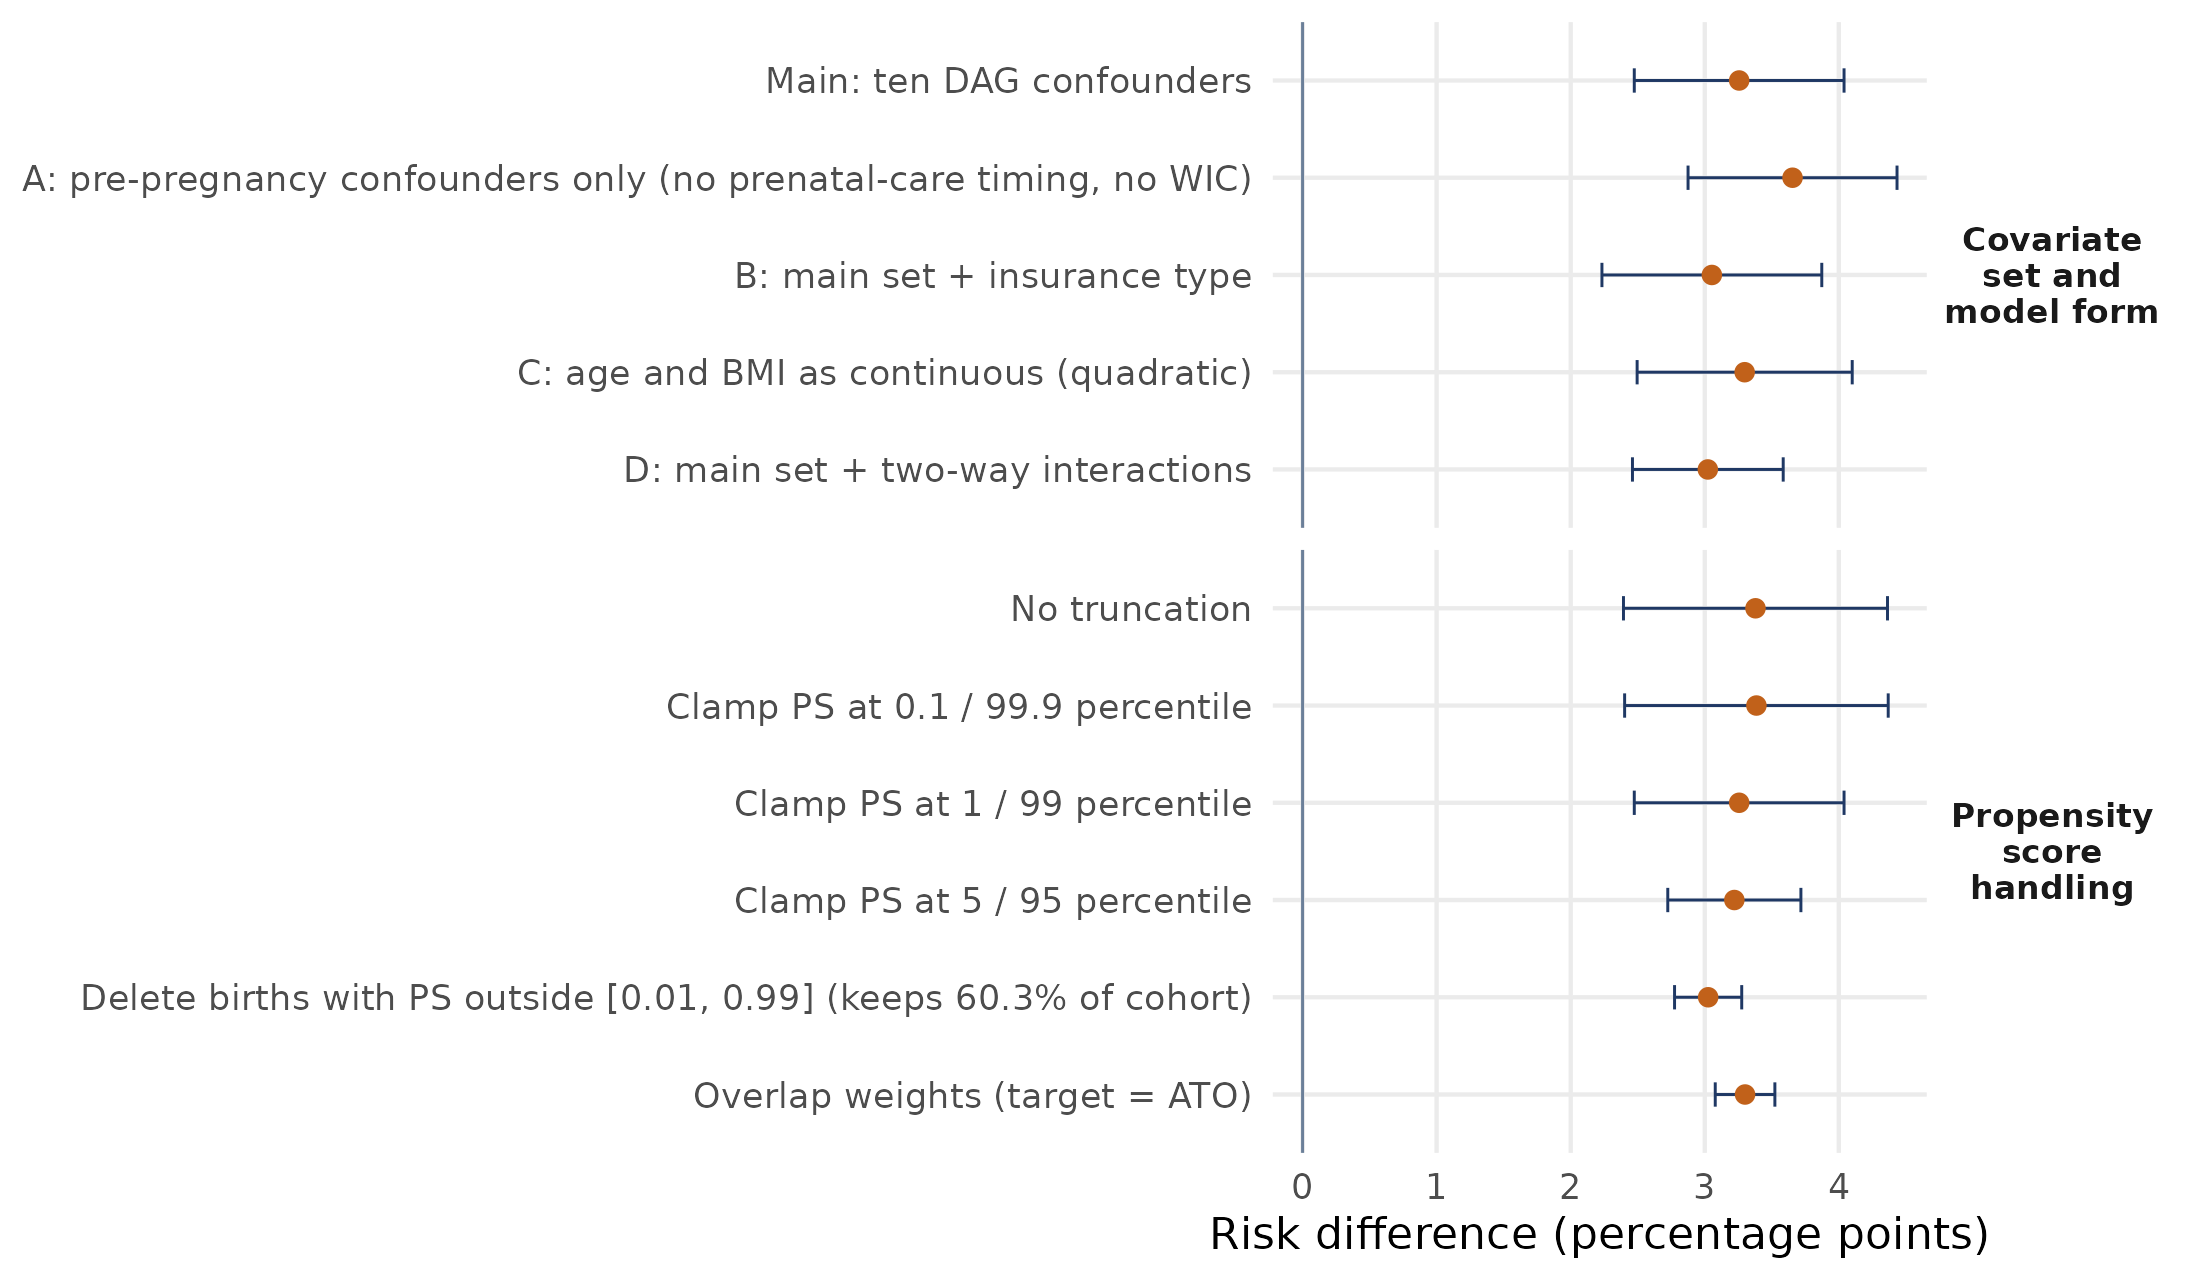
\includegraphics[width=5.6in]{figures/fig_robustness.png}
\caption*{\textbf{Figure 7.} \emph{AIPTW (and overlap-weighted) risk difference under alternative handling of the propensity score and alternative covariate specifications.}}
\end{figure}


\subsection*{6.5 Subgroups (exploratory)}

Subgroup AIPTW risk differences ranged from 0.90 to 5.53 percentage points (Figure 8), and the interval excluded zero in 24 of 29 subgroups. The point estimates were largest among Black mothers (5.0), mothers aged 35 to 39 (5.5), mothers with three or more previous births (5.2) and mothers with a normal pre-pregnancy BMI (4.6), and smallest among American Indian and Alaska Native mothers (0.9, interval -2.5 to 4.3), mothers with a BMI of 40 or more (1.2, interval -1.0 to 3.4), and mothers with a previous preterm birth (2.2 against 3.3 without). Previous preterm birth is also the level with the highest baseline risk (26.2 percent among non-smokers); no conclusion is drawn from this contrast. A subgroup estimate is the average of the same per-mother AIPTW values within the subgroup, intervals are wider for small groups, and with 29 subgroup estimates the pattern is treated as hypothesis-generating, not as evidence of effect modification. The full results are in the output file \texttt{subgroup\_aiptw.csv}.

\begin{figure}[htbp]
\centering
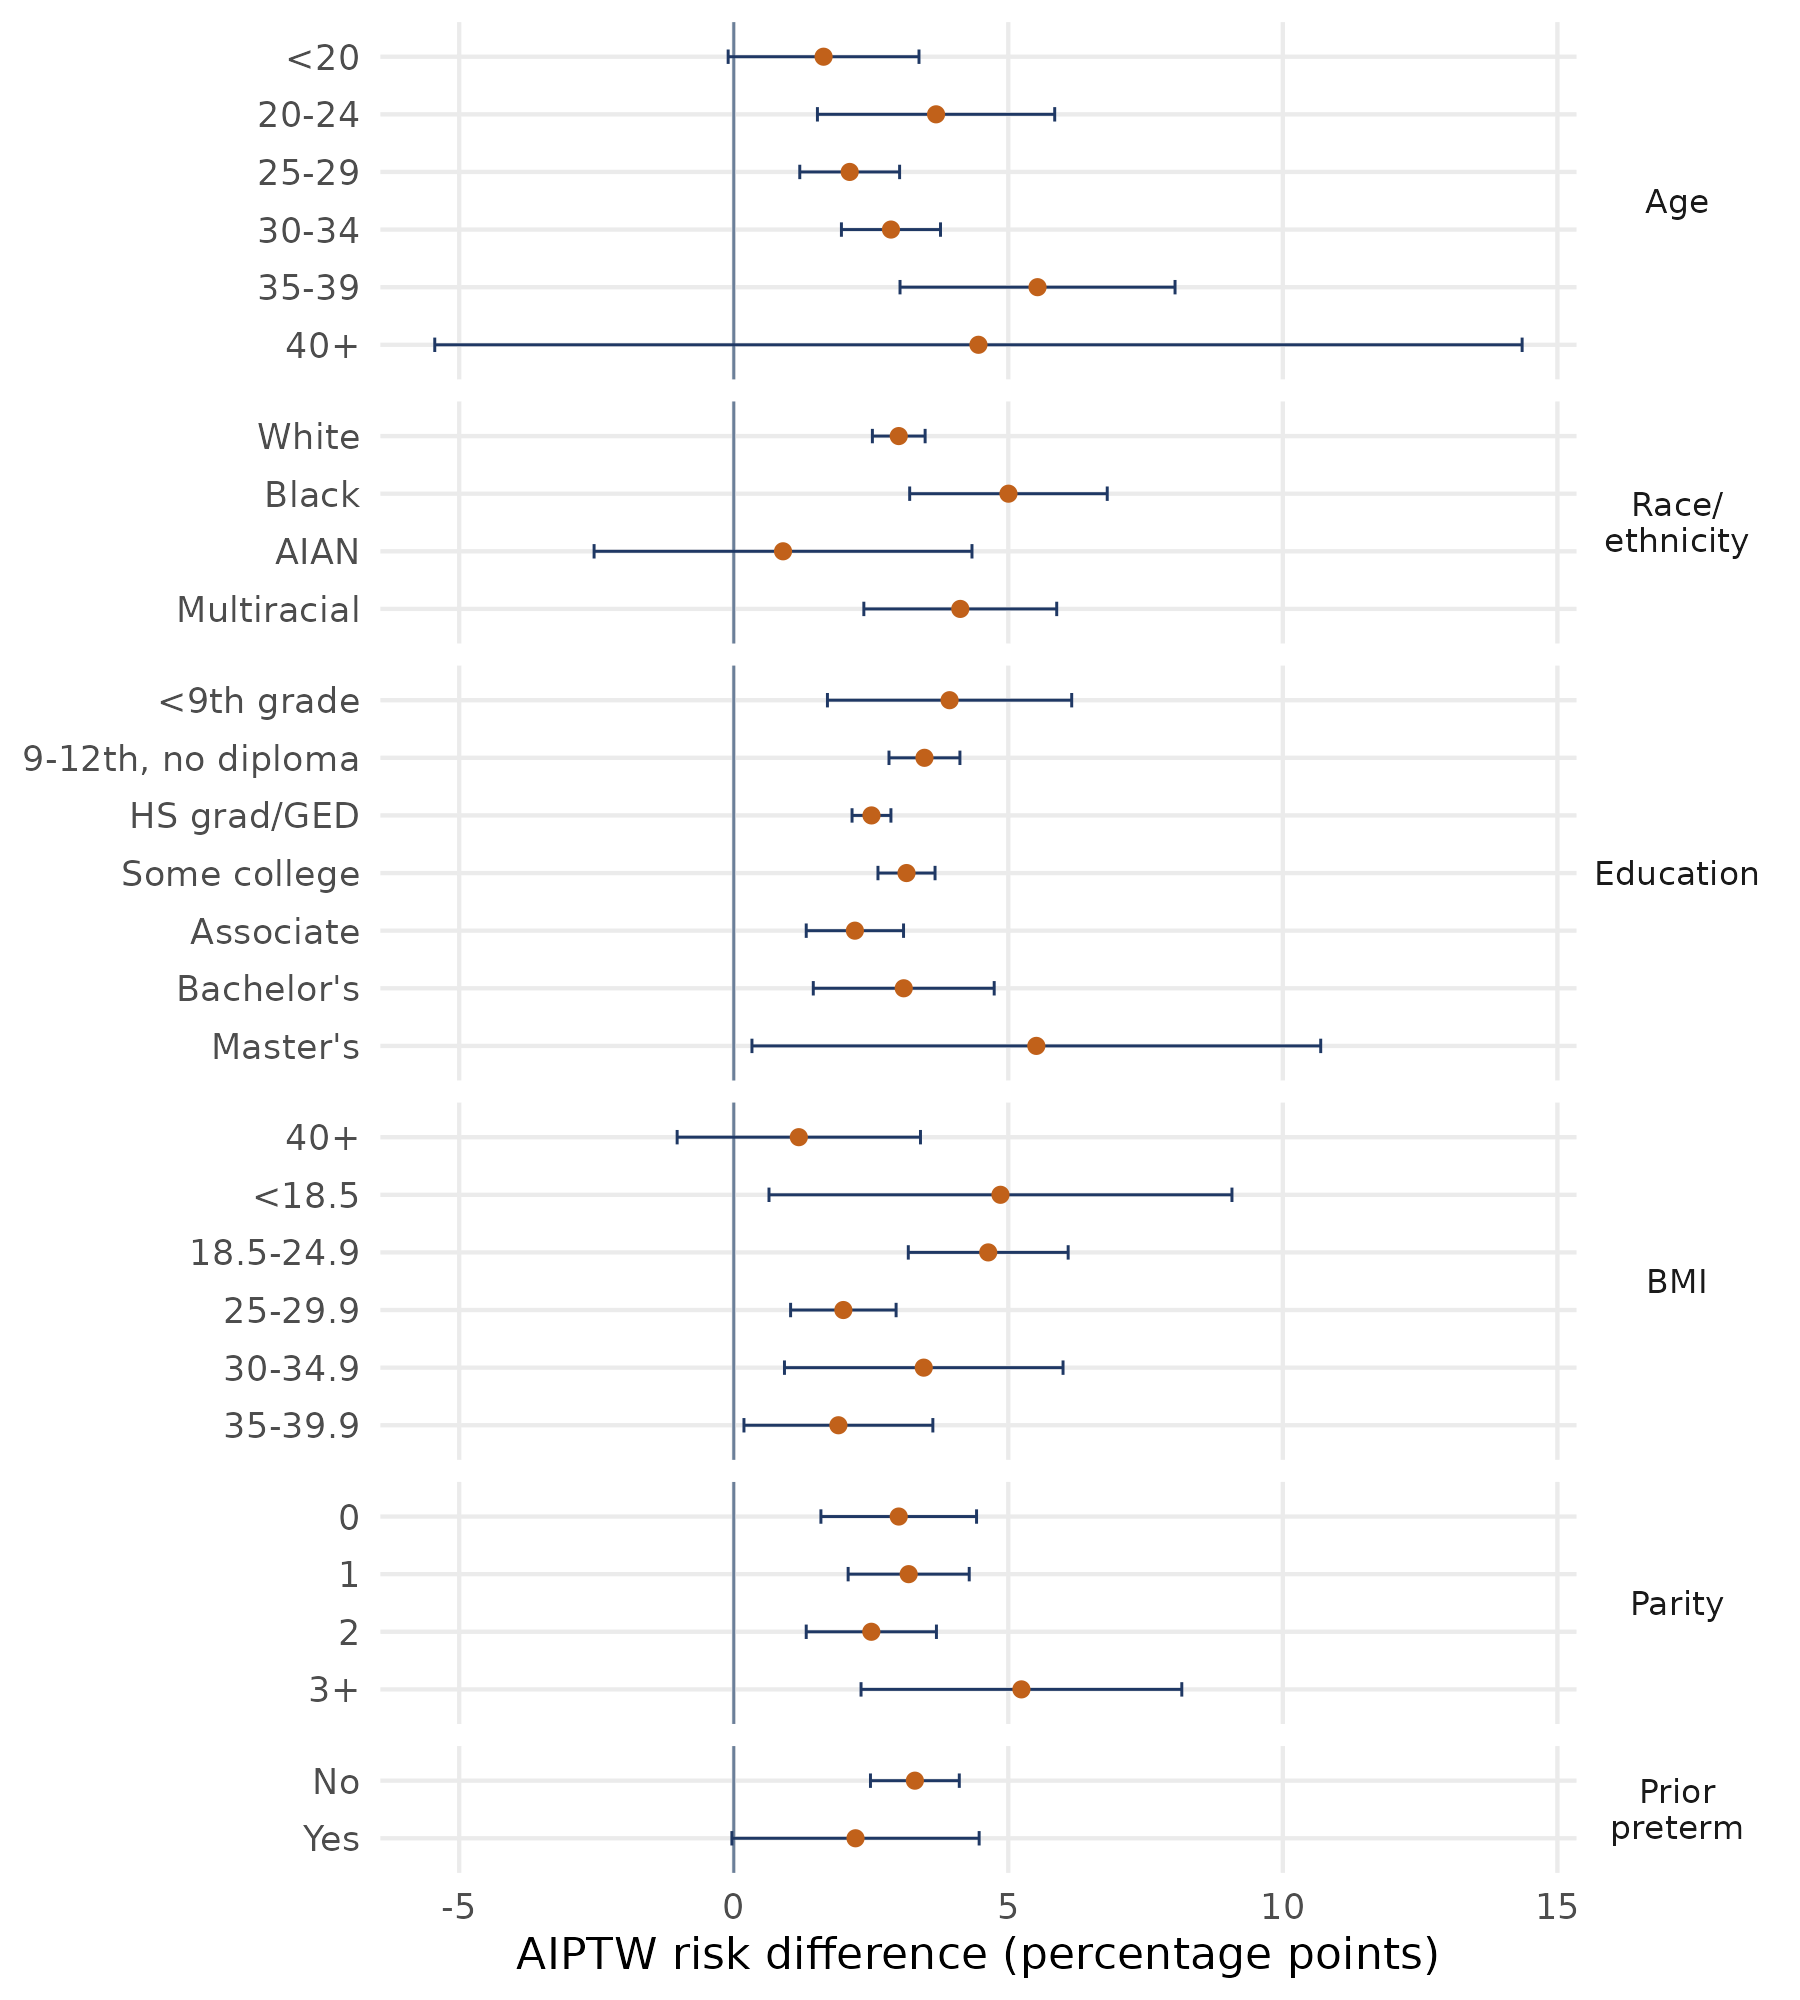
\includegraphics[width=4.6in]{figures/fig_subgroups.png}
\caption*{\textbf{Figure 8.} \emph{Exploratory AIPTW risk differences (percentage points, 95\% CI) within subgroups. Groups with fewer than 500 smokers are omitted.}}
\end{figure}


\subsection*{6.6 Check of the standard errors}

The closed-form standard errors were checked by repeating the whole pipeline (propensity model, outcome models, estimator) on 200 bootstrap resamples of a random subsample of 200,000 births (seed 1234). The subsample holds only about 6,000 smokers, so its point estimates (risk differences of 2.0 for AIPTW, 2.6 for stabilized IPTW, 1.8 for outcome regression) differ from the full-cohort values through sampling error; the purpose of this check is the standard errors, not the estimates. The ratio of the influence-function standard error to the bootstrap standard error was 1.17 for AIPTW (1.08 against 0.92 percentage points), 1.05 for stabilized IPTW (1.09 against 1.04 percentage points), 1.05 for outcome regression (0.69 against 0.66 percentage points). A ratio above one means that the closed-form standard error is larger than the bootstrap standard error. In this subsample the influence-function standard errors were not smaller than the bootstrap standard errors for any of the three estimators.

\section*{7. Discussion}

In the 2023 U.S. cohort, the AIPTW estimate of the effect of smoking during pregnancy on preterm birth was 3.3 percentage points (risk ratio 1.39), from 8.4 to 11.6 percent, under the assumptions in Section 4. This is 42 percent smaller than the crude difference of 5.6 points. The adjusted odds ratio of 1.44 lies within the range of 1.31 to 1.53 reported for first-trimester smoking by cigarettes per day in a regression analysis of 25.6 million U.S. births (Liu et al., 2020). The ATT of 3.4 points corresponds to about 34 additional preterm births per 1,000 smoking pregnancies, and its interval is narrower than that of the ATE.

Three features of the analysis bear on interpretation. First, overlap is weak for part of the cohort: 41 percent of non-smokers have an estimated probability of smoking below 0.01, and the largest weight among smokers was 187, so the ATE estimate depends on the few smokers with low estimated probabilities of smoking, who receive large weights. The estimates under the alternative propensity score handling rules (Table 5), including the overlap-weighted estimate, lie between 3.03 and 3.39 percentage points. Second, 3 covariate levels remain above the 0.10 threshold after weighting (Section 6.2). Third, the causal diagram is a set of assumptions, and Table 2 shows that for several arrows into smoking the supporting evidence is indirect. The E-value of 2.1 is the minimum risk ratio, with both smoking and preterm birth, that an unmeasured confounder would need to explain the estimate away; alcohol, cannabis, e-cigarette use, stress and interpregnancy interval are not measured in this file (Section 8), and the data do not show whether any of them reaches that strength. The estimates are therefore effects under the stated assumptions.

\section*{8. Limitations}

Smoking is self-reported on the birth certificate and is underreported. In eight states the revised certificate gave lower prenatal smoking than PRAMS (11.3 against 14.0 percent) (Tong et al., 2013b), in New York City and Vermont certificates recorded 10.4 percent against 14.1 percent in medical records (Howland et al., 2015), and pregnant smokers deny smoking more often than non-pregnant smokers when cotinine is measured (Dietz et al., 2011; Searles Nielsen et al., 2014). Non-differential misclassification of a binary exposure usually, but not always, biases toward the null (Jurek et al., 2005), whether underreporting differs by education or parity was not examined in these data. Gestational age from the obstetric estimate has been the NCHS measure since 2014 (Martin et al., 2015) and is not error free; disagreement with last-menstrual-period estimates is largest at 28 to 36 weeks, which is where most preterm births fall (Qin et al., 2008; Martin et al., 2015).

The file contains live births only. If smoking raises fetal loss, conditioning on live birth can bias exposure-outcome estimates in either direction (Leung et al., 2021; Liew et al., 2015; Neophytou et al., 2021), and this cannot be quantified with the data used. Birth certificates record clinical risk factors with low sensitivity (Reichman \& Hade, 2001; Vinikoor et al., 2010), so adjustment for diabetes, hypertension and previous preterm birth is subject to measurement error. Important confounders are unmeasured (alcohol, cannabis, e-cigarette use, stress, intimate partner violence, nutrition, interpregnancy interval, paternal factors) (Patra et al., 2011; Regan et al., 2021; Dole et al., 2003; Donovan et al., 2016; Ahrens et al., 2019). Prenatal-care timing and WIC are recorded during pregnancy and are subject to gestational age bias, and pre-pregnancy cigarettes per day and gestational conditions were not adjusted for; the first of these choices could leave residual confounding by a persistent smoking habit (Schisterman et al., 2009; Hernán et al., 2004). ``Any smoking'' combines doses and timing, so the estimate is an average over them. Complete cases (93.8 percent of the extract) were analysed; missingness was at most 2.2 percent for each variable, and whether it is random was not assessed. Overlap and the three unbalanced levels are discussed above. The results are for one national year, and the subgroup results are exploratory.

\section*{9. Conclusion and next steps}

In 3.26 million singleton births, the AIPTW estimate of the effect of smoking during pregnancy on preterm birth was a risk difference of 3.3 percentage points (95\% CI 2.5 to 4.0) and a risk ratio of 1.39, and 3.4 points among mothers who smoked, under the causal assumptions stated in Section 4. Estimates across alternative propensity score handling rules and covariate specifications ranged from 3.0 to 3.7 points. The estimates rest on limited overlap for some mothers, on self-reported exposure, and on assumptions that the E-value quantifies but cannot verify. Next steps are (1) flexible machine-learning nuisance models with cross-fitting inside the same AIPTW structure (Chernozhukov et al., 2018; Zivich \& Breskin, 2021); (2) dose, timing and cessation of smoking, which the binary exposure used here cannot separate; (3) pooling several birth years; and (4) a SAS implementation so that the analysis can be reproduced in the SAS environment of this conference.

\section*{Data and code availability}

The data are the public-use 2023 Natality file of the National Center for Health Statistics (\url{https://ftp.cdc.gov/pub/Health_Statistics/NCHS/Datasets/DVS/natality/Nat2023us.zip}, 224 MB, fixed-width; user guide at \url{https://ftp.cdc.gov/pub/Health_Statistics/NCHS/Dataset_Documentation/DVS/natality/UserGuide2023.pdf}). The analysis uses a 24-variable extract of 3,476,180 births that script \texttt{00\_extract\_data.R} rebuilds from the full file, and that is also supplied compressed (35.8 MB) with the code. All scripts run from a single folder in the order listed in Section 5.5, use set.seed(1234), and print their results; the run times are given at the top of each script.

\section*{Use of AI assistance}

The authors used an AI assistant (Claude, Anthropic) to organize and check the literature, to help write and test the R code, and to draft and edit text. The first author specified the question, the design and the analytic choices and ran the code. The numbers in this paper come directly from the code output, and the references were checked against journal, publisher or CDC records during preparation. Both authors are responsible for the content.

\section*{References}
{\small\setlength{\parindent}{-0.25in}\setlength{\leftskip}{0.25in}\setlength{\parskip}{3pt}
Ahrens, K. A., Nelson, H., Stidd, R. L., Moskosky, S., \& Hutcheon, J. A. (2019). Short interpregnancy intervals and adverse perinatal outcomes in high-resource settings: An updated systematic review. Paediatric and Perinatal Epidemiology, 33(1). \url{https://doi.org/10.1111/ppe.12503}

Aubin, H.-J., Farley, A., Lycett, D., Lahmek, P., \& Aveyard, P. (2012). Weight gain in smokers after quitting cigarettes: Meta-analysis. BMJ, 345. \url{https://doi.org/10.1136/bmj.e4439}

Austin, P. C., \& Stuart, E. A. (2015). Moving towards best practice when using inverse probability of treatment weighting (IPTW) using the propensity score to estimate causal treatment effects in observational studies. Statistics in Medicine, 34(28), 3661-3679. \url{https://doi.org/10.1002/sim.6607}

Bang, H., \& Robins, J. M. (2005). Doubly robust estimation in missing data and causal inference models. Biometrics, 61(4), 962-973. \url{https://doi.org/10.1111/j.1541-0420.2005.00377.x}

Bitler, M. P., \& Currie, J. (2005). Does WIC work? The effects of WIC on pregnancy and birth outcomes. Journal of Policy Analysis and Management, 24(1), 73-91. \url{https://doi.org/10.1002/pam.20070}

Borsari, L., Malagoli, C., Werler, M. M., Rothman, K. J., Malavolti, M., Rodolfi, R., De Girolamo, G., Nicolini, F., \& Vinceti, M. (2018). Joint effect of maternal tobacco smoking and pregestational diabetes on preterm births and congenital anomalies: A population-based study in Northern Italy. Journal of Diabetes Research. \url{https://doi.org/10.1155/2018/2782741}

Bramham, K., Parnell, B., Nelson-Piercy, C., Seed, P. T., Poston, L., \& Chappell, L. C. (2014). Chronic hypertension and pregnancy outcomes: Systematic review and meta-analysis. BMJ, 348, g2301. \url{https://doi.org/10.1136/bmj.g2301}

Brookhart, M. A., Schneeweiss, S., Rothman, K. J., Glynn, R. J., Avorn, J., \& Stürmer, T. (2006). Variable selection for propensity score models. American Journal of Epidemiology, 163(12), 1149-1156. \url{https://doi.org/10.1093/aje/kwj149}

Busso, M., DiNardo, J., \& McCrary, J. (2014). New evidence on the finite sample properties of propensity score reweighting and matching estimators. Review of Economics and Statistics, 96(5), 885-897. \url{https://doi.org/10.1162/REST_a_00431}

Carreras-Torres, R., Johansson, M., Haycock, P. C., Relton, C. L., Davey Smith, G., Brennan, P., \& Martin, R. M. (2018). Role of obesity in smoking behaviour: Mendelian randomisation study in UK Biobank. BMJ, 361, k1767. \url{https://doi.org/10.1136/bmj.k1767}

Chen, J., Sun, Y., Zhou, J., Meng, M., Zhou, F., He, J., \& Zou, G. (2026). Interaction between maternal smoking cessation timing and preexisting hypertension on fetal growth restriction: A nationwide population-based cohort study. Clinical Epidemiology. \url{https://doi.org/10.2147/CLEP.S596174}

Chernozhukov, V., Chetverikov, D., Demirer, M., Duflo, E., Hansen, C., Newey, W., \& Robins, J. (2018). Double/debiased machine learning for treatment and structural parameters. The Econometrics Journal, 21(1), C1-C68. \url{https://doi.org/10.1111/ectj.12097}

Cole, S. R., Platt, R. W., Schisterman, E. F., Chu, H., Westreich, D., Richardson, D., \& Poole, C. (2010). Illustrating bias due to conditioning on a collider. International Journal of Epidemiology, 39(2), 417-420. \url{https://doi.org/10.1093/ije/dyp334}

Dietz, P. M., Homa, D., England, L. J., Burley, K., Tong, V. T., Dube, S. R., \& Bernert, J. T. (2011). Estimates of nondisclosure of cigarette smoking among pregnant and nonpregnant women of reproductive age in the United States. American Journal of Epidemiology, 173(3), 355-359. \url{https://doi.org/10.1093/aje/kwq381}

Dole, N., Savitz, D. A., Hertz-Picciotto, I., Siega-Riz, A. M., McMahon, M. J., \& Buekens, P. (2003). Maternal stress and preterm birth. American Journal of Epidemiology, 157(1), 14-24.

Donovan, B. M., Spracklen, C. N., Schweizer, M. L., Ryckman, K. K., \& Saftlas, A. F. (2016). Intimate partner violence during pregnancy and the risk for adverse infant outcomes: A systematic review and meta-analysis. BJOG, 123(8), 1289-1299. \url{https://doi.org/10.1111/1471-0528.13928}

Drake, P., Driscoll, A. K., \& Mathews, T. J. (2018). Cigarette smoking during pregnancy: United States, 2016 (NCHS Data Brief No. 305). National Center for Health Statistics.

Driscoll, A. K., \& Gregory, E. C. W. (2020). Increases in prepregnancy obesity: United States, 2016-2019 (NCHS Data Brief No. 392). National Center for Health Statistics.

Duko, B., Gebremedhin, A. T., Tessema, G. A., Alati, R., \& Pereira, G. (2023). Average treatment effect of maternal prenatal tobacco smoking on offspring developmental vulnerability in early childhood. Annals of Epidemiology. \url{https://doi.org/10.1016/j.annepidem.2022.12.007}

Evans, W. N., \& Ringel, J. S. (1999). Can higher cigarette taxes improve birth outcomes? Journal of Public Economics, 72(1), 135-154.

Ferguson, K. D., McCann, M., Katikireddi, S. V., Thomson, H., Green, M. J., Smith, D. J., \& Lewsey, J. D. (2020). Evidence synthesis for constructing directed acyclic graphs (ESC-DAGs): A novel and systematic method for building directed acyclic graphs. International Journal of Epidemiology, 49, 322-329. \url{https://doi.org/10.1093/ije/dyz150}

Funk, M. J., Westreich, D., Wiesen, C., Stürmer, T., Brookhart, M. A., \& Davidian, M. (2011). Doubly robust estimation of causal effects. American Journal of Epidemiology, 173(7), 761-767. \url{https://doi.org/10.1093/aje/kwq439}

Gage, S. H., Bowden, J., Davey Smith, G., \& Munafo, M. R. (2018). Investigating causality in associations between education and smoking: A two-sample Mendelian randomization study. International Journal of Epidemiology. \url{https://doi.org/10.1093/ije/dyy131}

Ganchimeg, T., Ota, E., Morisaki, N., Laopaiboon, M., Lumbiganon, P., et al. (2014). Pregnancy and childbirth outcomes among adolescent mothers: A World Health Organization multicountry study. BJOG, 121(Suppl. 1), 40-48. \url{https://doi.org/10.1111/1471-0528.12630}

Gangopadhyaya, A., Dubay, L., Johnston, E., \& Pancini, V. (2024). How structural racism, neighborhood deprivation, and maternal characteristics contribute to inequities in birth outcomes. Health Affairs Scholar, 2(8), qxae092. \url{https://doi.org/10.1093/haschl/qxae092}

Goldenberg, R. L., Culhane, J. F., Iams, J. D., \& Romero, R. (2008). Epidemiology and causes of preterm birth. The Lancet, 371(9606), 75-84. \url{https://doi.org/10.1016/S0140-6736(08)60074-4}

Greenland, S., Pearl, J., \& Robins, J. M. (1999). Causal diagrams for epidemiologic research. Epidemiology, 10(1), 37-48. \url{https://doi.org/10.1097/00001648-199901000-00008}

Guh, D. P., Zhang, W., Bansback, N., Amarsi, Z., Birmingham, C. L., \& Anis, A. H. (2009). The incidence of co-morbidities related to obesity and overweight: A systematic review and meta-analysis. BMC Public Health, 9, 88. \url{https://doi.org/10.1186/1471-2458-9-88}

Heaman, M. I., Newburn-Cook, C. V., Green, C. G., Elliott, L. J., \& Helewa, M. E. (2008). Inadequate prenatal care and its association with adverse pregnancy outcomes: A comparison of indices. BMC Pregnancy and Childbirth, 8, 15. \url{https://doi.org/10.1186/1471-2393-8-15}

Heiny, E., \& Islam, M. (2026). Impact of maternal smoking during pregnancy on preterm birth risk in the United States [Invited e-poster abstract]. Joint Statistical Meetings 2026, Boston, MA.

Hernán, M. A., Hernández-Díaz, S., \& Robins, J. M. (2004). A structural approach to selection bias. Epidemiology, 15(5), 615-625. \url{https://doi.org/10.1097/01.ede.0000135174.63482.43}

Hiscock, R., Bauld, L., Amos, A., Fidler, J. A., \& Munafo, M. (2012). Socioeconomic status and smoking: A review. Annals of the New York Academy of Sciences, 1248(1), 107-123. \url{https://doi.org/10.1111/j.1749-6632.2011.06202.x}

Howland, R. E., Mulready-Ward, C., Madsen, A. M., Sackoff, J., Nyland-Funke, M., Bombard, J. M., \& Tong, V. T. (2015). Reliability of reported maternal smoking: Comparing the birth certificate to maternal worksheets and prenatal and hospital medical records, New York City and Vermont, 2009. Maternal and Child Health Journal, 19(9), 1916-1924. \url{https://doi.org/10.1007/s10995-015-1722-1}

Joyce, T., Racine, A., \& Yunzal-Butler, C. (2008). Reassessing the WIC effect: Evidence from the Pregnancy Nutrition Surveillance System. Journal of Policy Analysis and Management, 27(2), 277-303.

Juárez, S. P., \& Merlo, J. (2013). Revisiting the effect of maternal smoking during pregnancy on offspring birthweight: A quasi-experimental sibling analysis in Sweden. PLOS ONE. \url{https://doi.org/10.1371/journal.pone.0061734}

Jurek, A. M., Greenland, S., Maldonado, G., \& Church, T. R. (2005). Proper interpretation of non-differential misclassification effects: Expectations vs observations. International Journal of Epidemiology, 34(3), 680-687. \url{https://doi.org/10.1093/ije/dyi060}

Kang, J. D. Y., \& Schafer, J. L. (2007). Demystifying double robustness: A comparison of alternative strategies for estimating a population mean from incomplete data. Statistical Science, 22(4). \url{https://doi.org/10.1214/07-STS227}

Kazemier, B. M., Buijs, P. E., Mignini, L., Limpens, J., de Groot, C. J. M., Mol, B. W. J., \& Oude Rengerink, K. (2014). Impact of obstetric history on the risk of spontaneous preterm birth in singleton and multiple pregnancies: A systematic review. BJOG. \url{https://doi.org/10.1111/1471-0528.12896}

King, G., \& Nielsen, R. (2019). Why propensity scores should not be used for matching. Political Analysis, 27(4), 435-454. \url{https://doi.org/10.1017/pan.2019.11}

Kondracki, A. J. (2019). Prevalence and patterns of cigarette smoking before and during early and late pregnancy according to maternal characteristics: The first national data based on the 2003 birth certificate revision, United States, 2016. Reproductive Health, 16. \url{https://doi.org/10.1186/s12978-019-0807-5}

Koullali, B., van Zijl, M. D., Kazemier, B. M., Oudijk, M. A., Mol, B. W. J., Pajkrt, E., \& Ravelli, A. C. J. (2020). The association between parity and spontaneous preterm birth: A population based study. BMC Pregnancy and Childbirth. \url{https://doi.org/10.1186/s12884-020-02940-w}

Kozuki, N., Lee, A. C., Silveira, M. F., Victora, C. G., Adair, L., Humphrey, J., ... Katz, J. (2013). The associations of parity and maternal age with small-for-gestational-age, preterm, and neonatal and infant mortality: A meta-analysis. BMC Public Health, 13(Suppl 3), S2.

Lee, B. K., Lessler, J., \& Stuart, E. A. (2011). Weight trimming and propensity score weighting. PLoS ONE, 6(3), e18174. \url{https://doi.org/10.1371/journal.pone.0018174}

Leung, M., Kioumourtzoglou, M.-A., Raz, R., \& Weisskopf, M. G. (2021). Bias due to selection on live births in studies of environmental exposures during pregnancy: A simulation study. Environmental Health Perspectives, 129(4), 047001. \url{https://doi.org/10.1289/EHP7961}

Li, F., Morgan, K. L., \& Zaslavsky, A. M. (2018). Balancing covariates via propensity score weighting. Journal of the American Statistical Association, 113(521), 390-400. \url{https://doi.org/10.1080/01621459.2016.1260466}

Liew, Z., Olsen, J., Cui, X., Ritz, B., \& Arah, O. A. (2015). Bias from conditioning on live birth in pregnancy cohorts: An illustration based on neurodevelopment in children after prenatal exposure to organic pollutants. International Journal of Epidemiology, 44(1), 345-354. \url{https://doi.org/10.1093/ije/dyu249}

Liu, B., Xu, G., Sun, Y., Qiu, X., Ryckman, K. K., Yu, Y., Snetselaar, L. G., \& Bao, W. (2020). Maternal cigarette smoking before and during pregnancy and the risk of preterm birth: A dose-response analysis of 25 million mother-infant pairs. PLOS Medicine, 17(8), e1003158. \url{https://doi.org/10.1371/journal.pmed.1003158}

Martin, J. A., Hamilton, B. E., \& Osterman, M. J. K. (2018). Births in the United States, 2017 (NCHS Data Brief No. 318). National Center for Health Statistics.

Martin, J. A., Osterman, M. J. K., Kirmeyer, S. E., \& Gregory, E. C. W. (2015). Measuring gestational age in vital statistics data: Transitioning to the obstetric estimate. National Vital Statistics Reports, 64(5).

Mathews, T. J., \& Hamilton, B. E. (2016). Mean age of mothers is on the rise: United States, 2000-2014 (NCHS Data Brief No. 232). National Center for Health Statistics.

McDonald, S. D., Han, Z., Mulla, S., \& Beyene, J. (2010). Overweight and obesity in mothers and risk of preterm birth and low birth weight infants: Systematic review and meta-analyses. BMJ, c3428.

Moore, E., Blatt, K., Chen, A., Van Hook, J., \& DeFranco, E. A. (2016). Factors associated with smoking cessation in pregnancy. American Journal of Perinatology. \url{https://doi.org/10.1055/s-0035-1570319}

Murphy, H. R., Howgate, C., O'Keefe, J., et al. (2021). Characteristics and outcomes of pregnant women with type 1 or type 2 diabetes: A 5-year national population-based cohort study. The Lancet Diabetes \& Endocrinology.

Naimi, A. I., Cole, S. R., \& Kennedy, E. H. (2017). An introduction to g methods. International Journal of Epidemiology, 46(2), 756-762. \url{https://doi.org/10.1093/ije/dyw323}

National Center for Education Statistics. (2023). Educational attainment of young adults (Condition of Education). U.S. Department of Education. \url{https://nces.ed.gov/programs/coe/indicator/caa}

National Center for Health Statistics. (2024). User guide to the 2023 natality public use file. \url{https://ftp.cdc.gov/pub/Health_Statistics/NCHS/Dataset_Documentation/DVS/natality/UserGuide2023.pdf}

Neophytou, A. M., Kioumourtzoglou, M.-A., Goin, D. E., Darwin, K. C., \& Casey, J. A. (2021). Educational note: Addressing special cases of bias that frequently occur in perinatal epidemiology. International Journal of Epidemiology, 50(1), 337-345. \url{https://doi.org/10.1093/ije/dyaa252}

Osterman, M. J. K., Hamilton, B. E., Martin, J. A., Driscoll, A. K., \& Valenzuela, C. P. (2025). Births: Final data for 2023. National Vital Statistics Reports, 74(1). National Center for Health Statistics.

Patra, J., Bakker, R., Irving, H., Jaddoe, V. W. V., Malini, S., \& Rehm, J. (2011). Dose-response relationship between alcohol consumption before and during pregnancy and the risks of low birthweight, preterm birth and small for gestational age (SGA): A systematic review and meta-analyses. BJOG, 118(12), 1411-1421. \url{https://doi.org/10.1111/j.1471-0528.2011.03050.x}

Pearl, J. (1995). Causal diagrams for empirical research. Biometrika, 82(4), 669-688. \url{https://doi.org/10.1093/biomet/82.4.669}

Phelan, J. C., \& Link, B. G. (2015). Is racism a fundamental cause of inequalities in health? Annual Review of Sociology, 41, 311-330. \url{https://doi.org/10.1146/annurev-soc-073014-112305}

Philips, E. M., Santos, S., Trasande, L., Aurrekoetxea, J. J., Barros, H., von Berg, A., ... Jaddoe, V. W. V. (2020). Changes in parental smoking during pregnancy and risks of adverse birth outcomes and childhood overweight in Europe and North America: An individual participant data meta-analysis of 229,000 singleton births. PLOS Medicine. \url{https://doi.org/10.1371/journal.pmed.1003182}

Qin, C., Hsia, J., \& Berg, C. J. (2008). Variation between last-menstrual-period and clinical estimates of gestational age in vital records. American Journal of Epidemiology, 167(6), 646-652.

Regan, A. K., Bombard, J. M., O'Hegarty, M. M., Smith, R. A., \& Tong, V. T. (2021). Adverse birth outcomes associated with prepregnancy and prenatal electronic cigarette use. Obstetrics \& Gynecology, 138(1), 85-94. \url{https://doi.org/10.1097/AOG.0000000000004432}

Reichman, N. E., \& Hade, E. M. (2001). Validation of birth certificate data: A study of women in New Jersey's HealthStart program. Annals of Epidemiology, 11(3), 186-193.

Robins, J. M., Rotnitzky, A., \& Zhao, L. P. (1994). Estimation of regression coefficients when some regressors are not always observed. Journal of the American Statistical Association, 89(427), 846-866. \url{https://doi.org/10.1080/01621459.1994.10476818}

Rosenbaum, P. R., \& Rubin, D. B. (1983). The central role of the propensity score in observational studies for causal effects. Biometrika, 70(1), 41-55. \url{https://doi.org/10.1093/biomet/70.1.41}

Rosenbaum, P. R., \& Rubin, D. B. (1984). Reducing bias in observational studies using subclassification on the propensity score. Journal of the American Statistical Association, 79(387), 516-524. \url{https://doi.org/10.1080/01621459.1984.10478078}

Rubin, D. B. (1974). Estimating causal effects of treatments in randomized and nonrandomized studies. Journal of Educational Psychology, 66(5), 688-701. \url{https://doi.org/10.1037/h0037350}

Ruiz, M., Goldblatt, P., Morrison, J., Kukla, L., Svancara, J., et al. (2015). Mother's education and the risk of preterm and small for gestational age birth: A DRIVERS meta-analysis of 12 European cohorts. Journal of Epidemiology and Community Health, 69(9), 826-833. \url{https://doi.org/10.1136/jech-2014-205387}

Schisterman, E. F., Cole, S. R., \& Platt, R. W. (2009). Overadjustment bias and unnecessary adjustment in epidemiologic studies. Epidemiology, 20(4), 488-495. \url{https://doi.org/10.1097/EDE.0b013e3181a819a1}

Searles Nielsen, S., Dills, R. L., Glass, M., \& Mueller, B. A. (2014). Accuracy of prenatal smoking data from Washington State birth certificates in a population-based sample with cotinine measurements. Annals of Epidemiology, 24(3). \url{https://doi.org/10.1016/j.annepidem.2013.12.008}

Shah, N. R., \& Bracken, M. B. (2000). A systematic review and meta-analysis of prospective studies on the association between maternal cigarette smoking and preterm delivery. American Journal of Obstetrics and Gynecology, 182, 465-472. \url{https://doi.org/10.1016/s0002-9378(00)70240-7}

Shin, D., \& Song, W. O. (2019). Influence of the adequacy of the Prenatal Care Utilization Index on small-for-gestational-age infants and preterm births in the United States. Journal of Clinical Medicine, 8(6), 838. \url{https://doi.org/10.3390/jcm8060838}

Stock, S. J., \& Bauld, L. (2020). Maternal smoking and preterm birth: An unresolved health challenge. PLOS Medicine. \url{https://doi.org/10.1371/journal.pmed.1003386}

Stoner, M. C. D., Cole, S. R., Price, J. T., Winston, J. J., \& Stringer, J. S. A. (2018). Timing of initiation of antiretroviral therapy and risk of preterm birth in studies of HIV-infected pregnant women: The role of selection bias. Epidemiology. \url{https://doi.org/10.1097/ede.0000000000000772}

Stuart, E. A. (2010). Matching methods for causal inference: A review and a look forward. Statistical Science, 25(1). \url{https://doi.org/10.1214/09-STS313}

Tennant, P. W. G., Murray, E. J., Arnold, K. F., Berrie, L., Fox, M. P., Gadd, S. C., ... Ellison, G. T. H. (2021). Use of directed acyclic graphs (DAGs) to identify confounders in applied health research: Review and recommendations. International Journal of Epidemiology, 50(2), 620-632. \url{https://doi.org/10.1093/ije/dyaa213}

Tong, V. T., Dietz, P. M., Farr, S. L., D'Angelo, D. V., \& England, L. J. (2013). Estimates of smoking before and during pregnancy, and smoking cessation during pregnancy: Comparing two population-based data sources. Public Health Reports, 128(3), 179-188.

Tong, V. T., Dietz, P. M., Morrow, B., D'Angelo, D. V., Farr, S. L., Rockhill, K. M., \& England, L. J. (2013). Trends in smoking before, during, and after pregnancy: Pregnancy Risk Assessment Monitoring System, United States, 40 sites, 2000-2010. MMWR Surveillance Summaries, 62(SS-6).

Torloni, M. R., Betran, A. P., Daher, S., Widmer, M., Dolan, S. M., Menon, R., Bergel, E., Allen, T., \& Merialdi, M. (2009). Maternal BMI and preterm birth: A systematic review of the literature with meta-analysis. Journal of Maternal-Fetal and Neonatal Medicine. \url{https://doi.org/10.3109/14767050903042561}

U.S. Department of Agriculture, Food and Nutrition Service. (n.d.). WIC eligibility. \url{https://www.fns.usda.gov/wic/eligibility}

VanderWeele, T. J., \& Ding, P. (2017). Sensitivity analysis in observational research: Introducing the E-value. Annals of Internal Medicine, 167(4), 268-274. \url{https://doi.org/10.7326/M16-2607}

VanderWeele, T. J., \& Robinson, W. R. (2014). On the causal interpretation of race in regressions adjusting for confounding and mediating variables. Epidemiology, 25, 473-484. \url{https://doi.org/10.1097/EDE.0000000000000105}

VanderWeele, T. J., \& Shpitser, I. (2011). A new criterion for confounder selection. Biometrics, 67(4), 1406-1413. \url{https://doi.org/10.1111/j.1541-0420.2011.01619.x}

Veiga, P. V., \& Wilder, R. P. (2008). Maternal smoking during pregnancy and birthweight: A propensity score matching approach. Maternal and Child Health Journal, 12(2). \url{https://doi.org/10.1007/s10995-007-0238-8}

Vinikoor, L. C., Messer, L. C., Laraia, B. A., \& Kaufman, J. S. (2010). Reliability of variables on the North Carolina birth certificate: A comparison with directly queried values from a cohort study. Paediatric and Perinatal Epidemiology, 24(1), 102-112.

Yunzal-Butler, C., Joyce, T. J., \& Racine, A. D. (2009). Maternal smoking and the timing of WIC enrollment (NBER Working Paper No. 14728). National Bureau of Economic Research. \url{https://doi.org/10.3386/w14728}

Zivich, P. N., \& Breskin, A. (2021). Machine learning for causal inference: On the use of cross-fit estimators. Epidemiology, 32(3), 393-401. \url{https://doi.org/10.1097/EDE.0000000000001332}

}
\section*{Appendix}
{\scriptsize
\begin{longtable}{>{\raggedright\arraybackslash}p{0.183\textwidth}>{\raggedright\arraybackslash}p{0.231\textwidth}>{\raggedright\arraybackslash}p{0.168\textwidth}>{\raggedright\arraybackslash}p{0.144\textwidth}>{\raggedright\arraybackslash}p{0.087\textwidth}>{\raggedright\arraybackslash}p{0.088\textwidth}}
\caption*{\textbf{Table A1.} \emph{Characteristics of the analytic cohort by smoking status, and crude preterm birth risk (\%) within each level. Column percentages are within smoking group.}}\\
\toprule
\rowcolor{headgray} \textbf{Variable} & \textbf{Level} & \textbf{Non-smokers n (\%)} & \textbf{Smokers n (\%)} & \textbf{Preterm \% non-smokers} & \textbf{Preterm \% smokers} \\
\midrule
\endfirsthead
\toprule
\rowcolor{headgray} \textbf{Variable} & \textbf{Level} & \textbf{Non-smokers n (\%)} & \textbf{Smokers n (\%)} & \textbf{Preterm \% non-smokers} & \textbf{Preterm \% smokers} \\
\midrule
\endhead
\bottomrule
\endfoot
Maternal age (years) & <20 & 126,638 (4.0) & 2,922 (3.0) & 9.7 & 11.8 \\
 & 20-24 & 544,546 (17.2) & 18,956 (19.5) & 8.1 & 10.9 \\
 & 25-29 & 870,584 (27.5) & 28,230 (29.0) & 7.6 & 11.9 \\
 & 30-34 & 966,655 (30.6) & 28,721 (29.6) & 7.8 & 14.4 \\
 & 35-39 & 527,652 (16.7) & 14,855 (15.3) & 9.2 & 19.0 \\
 & 40+ & 126,234 (4.0) & 3,503 (3.6) & 12.2 & 21.8 \\
Race/ethnicity & White & 2,346,025 (74.2) & 77,382 (79.6) & 7.7 & 13.0 \\
 & Black & 481,211 (15.2) & 12,376 (12.7) & 11.6 & 19.2 \\
 & AIAN & 28,932 (0.9) & 2,282 (2.3) & 9.5 & 13.6 \\
 & Asian & 202,949 (6.4) & 418 (0.4) & 7.6 & 14.4 \\
 & NHOPI & 11,707 (0.4) & 177 (0.2) & 10.0 & 11.3 \\
 & Multiracial & 91,485 (2.9) & 4,552 (4.7) & 8.5 & 15.4 \\
Education & <9th grade & 102,634 (3.2) & 1,948 (2.0) & 8.5 & 16.2 \\
 & 9-12th, no diploma & 232,495 (7.4) & 21,434 (22.1) & 10.3 & 15.2 \\
 & HS grad/GED & 831,985 (26.3) & 44,482 (45.8) & 9.3 & 13.3 \\
 & Some college & 543,999 (17.2) & 20,739 (21.3) & 9.1 & 14.0 \\
 & Associate & 268,066 (8.5) & 5,268 (5.4) & 8.6 & 13.7 \\
 & Bachelor's & 731,502 (23.1) & 2,688 (2.8) & 6.8 & 11.9 \\
 & Master's & 347,646 (11.0) & 547 (0.6) & 6.8 & 13.7 \\
 & Doctorate/Prof. & 103,982 (3.3) & 81 (0.1) & 6.7 & 12.3 \\
Prenatal care began & 1st trimester & 2,439,888 (77.2) & 61,460 (63.2) & 8.2 & 12.2 \\
 & 2nd trimester & 522,024 (16.5) & 22,580 (23.2) & 7.8 & 13.5 \\
 & 3rd trimester & 142,354 (4.5) & 7,527 (7.7) & 6.6 & 12.2 \\
 & No care & 58,043 (1.8) & 5,620 (5.8) & 20.3 & 36.7 \\
WIC & No & 2,191,695 (69.3) & 45,782 (47.1) & 8.0 & 15.6 \\
 & Yes & 970,614 (30.7) & 51,405 (52.9) & 9.0 & 12.4 \\
Parity (previous live births) & 0 & 1,291,042 (40.8) & 24,099 (24.8) & 8.5 & 13.2 \\
 & 1 & 985,650 (31.2) & 26,063 (26.8) & 7.1 & 12.3 \\
 & 2 & 507,264 (16.0) & 21,507 (22.1) & 8.3 & 12.8 \\
 & 3+ & 378,353 (12.0) & 25,518 (26.3) & 10.7 & 17.1 \\
Previous preterm birth & No & 3,044,731 (96.3) & 88,555 (91.1) & 7.6 & 12.2 \\
 & Yes & 117,578 (3.7) & 8,632 (8.9) & 26.1 & 31.1 \\
Pre-pregnancy diabetes & No & 3,123,571 (98.8) & 95,459 (98.2) & 8.1 & 13.5 \\
 & Yes & 38,738 (1.2) & 1,728 (1.8) & 26.1 & 33.8 \\
Pre-pregnancy hypertension & No & 3,065,467 (96.9) & 92,081 (94.7) & 7.9 & 13.3 \\
 & Yes & 96,842 (3.1) & 5,106 (5.3) & 19.9 & 25.0 \\
Pre-pregnancy BMI & <18.5 & 82,622 (2.6) & 4,766 (4.9) & 9.7 & 17.7 \\
 & 18.5-24.9 & 1,193,962 (37.8) & 33,295 (34.3) & 7.1 & 15.1 \\
 & 25-29.9 & 880,286 (27.8) & 23,359 (24.0) & 7.8 & 13.1 \\
 & 30-34.9 & 537,854 (17.0) & 17,126 (17.6) & 9.1 & 12.6 \\
 & 35-39.9 & 271,392 (8.6) & 10,087 (10.4) & 10.4 & 12.7 \\
 & 40+ & 196,193 (6.2) & 8,554 (8.8) & 12.5 & 13.5 \\
\end{longtable}
}

\end{document}
